\documentclass[11pt]{article}
\usepackage[utf8]{inputenc}
\usepackage{amsmath,amsthm,amsfonts,amssymb,amscd}
\usepackage{multirow,booktabs}
\usepackage[table]{xcolor}
\usepackage{fullpage}
\usepackage{lastpage}
\usepackage{enumitem}
\usepackage{fancyhdr}
\usepackage{mathrsfs}
\usepackage{wrapfig}
\usepackage{setspace}
\usepackage{calc}
\usepackage{multicol}
\usepackage{cancel}
\usepackage[retainorgcmds]{IEEEtrantools}
\usepackage[margin=3cm]{geometry}
\usepackage{amsmath}
\newlength{\tabcont}
\setlength{\parindent}{0.0in}
\setlength{\parskip}{0.05in}
\usepackage{empheq}
\usepackage{framed}
\usepackage[most]{tcolorbox}
\usepackage{xcolor}
\colorlet{shadecolor}{orange!15}
\parindent 0in
\parskip 12pt
\geometry{margin=1in, headsep=0.25in}
\theoremstyle{definition}
\newtheorem{defn}{Definition}
\newtheorem{reg}{Rule}
\newtheorem{exer}{Exercise}
\newtheorem{note}{Note}
\usepackage{listings}
\usepackage{xcolor}
\usepackage{graphicx}
\setlist[itemize]{noitemsep, topsep=0pt}
\setlength{\OuterFrameSep}{0pt}
\graphicspath{ {./images/} }
\newcommand{\N}{\mathbb{N}}
\newcommand{\Z}{\mathbb{Z}}
\newcommand{\C}{\mathbb{C}}
\newcommand{\R}{\mathbb{R}}
\newcommand*{\Co}[2]{{}^{#1}C_{#2}}%
\lstset { %
    language=C++,
    backgroundcolor=\color{black!5}, % set backgroundcolor
    basicstyle=\footnotesize,% basic font setting
}
\NewDocumentCommand{\codeword}{v}{%
\texttt{\textbf{#1}}%
}
\begin{document}
\title{Review}
\thispagestyle{empty}

\begin{center}
{\vspace{5mm} \LARGE ECE 205 - Fall 2018 \\ \vspace{5mm}Aditya Arora\\ \vspace{5mm} 6th September 2018}\\
{\vspace{5mm} \LARGE \bf Week 1 - Review \& Introduction}

\end{center}

\section{Complex Numbers}
Mathematics: $"i" = \sqrt{-1}$\\
Engineering: $"j" = \sqrt{-1}$
\subsection{Euler Formula}
$$e^{j\theta} = cos\theta + jsin\theta$$
We will have expression of the form $e^mt$ where m satisfies $am^2 + bm + c = 0$
\subsubsection{Real Roots}
If $am^2 + bm + c = 0$ has real roots $r_1, r_2$ then that leads to solutions $e^{r_1t}, e^{r_2t}$\\
We often take linear combinations of those solutions: $a_1e^{r_1t} + a_2e^{r_2t}$

\subsubsection{Complex Roots}
If $am^2 + bm + c = 0$ has complex roots $\alpha + j\beta, \alpha - j\beta, \;(\alpha,\: \beta\: \epsilon\: \R)$ then that leads to functions $e^{(\alpha + j\beta)t}, e^{(\alpha - j\beta)t}$\\
We also take linear combinations of those solutions: $$\frac{1}{2}[e^{(\alpha + j\beta)t} + e^{(\alpha - j\beta)t}] = e^{\alpha t}cos\beta t$$ because the complex component cancels out from Euler's formula. \\
Similarly taking a complex linear combination, $$\frac{1}{2j}[e^{(\alpha + j\beta)t} - e^{(\alpha - j\beta)t}] = e^{\alpha t}sin\beta t$$
Taking a real linear combination, we will have a solution of the form
$$Ae^{\alpha t}cos\beta t + Be^{\alpha t}sin\beta t \; (A,\:B\: \epsilon\: \R)$$

\section{Linear Algebra}
Everything is set up to manage and use Vector Spaces as $\R^n, M_{m+n} \; P_3$
\subsection{Linear Equation}
$$A\vec{x} = \vec{b}$$
$A\:  \epsilon\:  M_{m+n}\: [known],\: b\: \epsilon\: \R^n\:  [unknown],\: b\: \epsilon\:  \R^m\:  [known]$
\subsubsection{Special Cases}
Homogeneous Equation:$A\vec{x} = \vec{0}_{\R^m}$\\
$\vec{0}_{\R^n}$ is a solution\\
A solution set \textbf{$S$} is a vector subspace of $\R^n$\\
If $\vec{x}_1, \vec{x}_2 \epsilon S$ then $\vec{x}_1 + \vec{x}_2 \epsilon S$ and if $\vec{x}_1 \epsilon S $ then $ c\vec{x}_1 \epsilon S$
\subsubsection{Some other points}
Consider In-homogeneous equation $$A\vec{x} = \vec{b}$$
$\vec{b} \neq \vec{0}$ with  solution set $\tilde{S}$
\begin{enumerate}
    \item Lemma 1: Let $\vec{y_1}\; \epsilon\; \tilde{S}$ and $\vec{y_2}\; \epsilon\; \tilde{S}$\\
    Then $\vec{y_1}\; -\; \vec{y_2}\; \epsilon\; S$\\
    Moreover $\vec{y_1}\; -\; \vec{y_2}\; =\; \vec{x_1}$ where $\vec{x_1}\; \epsilon\; S$ then $\vec{y_1}\; =\; \vec{x_1}\; +\; \vec{y_2}$
    \item Lemma 2: We can obtain $\tilde{S}$ by finding one solution $\vec{y_2}\; \epsilon\; \tilde{S}$ [a particular solution] and then add it to each and every solution in set $S$ one by one\\
    If there are no solutions i.e. you cannot obtain $\vec{y_2}$, then $\tilde{S}$ is empty
\end{enumerate}
\newpage
\begin{center}
    {\LARGE 7th September 2018 \\ Lecture 1}
\end{center}
\setcounter{section}{0}
\section{Differential Equations}
\subsection{Introduction}
In calculus we deal with functions sometimes the functions are provided explicitly, however often we only have information about derivatives(s) of the function. \textit{Eg:} Newtown's law in 1 dimension, with constant mass: $$F = \frac{d\vec{p}}{dt}$$
Using momentum as $\vec{p} = m \vec{v} = m\frac{dx}{dt}$
$$F = m\frac{d^2x}{dt^2}$$
\textit{Eg:} one dimensional Motion under gravity, $g = \frac{d^2x}{dt^2} = 9.81ms^{-2}$
$$F = m\vec{a} = m\vec{g}$$

\subsubsection{Definitions and Vocabulary}
There are many types and we need some vocabulary to distinguish between them\\
\textbf{Def \#1:} A differential equation [DE] is an equation which involves the derivative(s) of some unknown function(s).\\
\textbf{Def \#2:} When we have a DE we will have one (or more) function(s) which we are trying to determine. This function(s) is(are) called the dependent variable(s). The other variables are called independent variables.\\
\textit{Eg:} $\frac{d^2x}{dt^2} = g$, $g$ is constant, $x$ is the dependent variable, $t$ is the independent variable\\
\textit{Eg:} $c\frac{\partial^2z}{\partial x^2} = \frac{\partial^2z}{\partial t^2}$, $c$ is constant, $z$ is the dependent variable, $t, x$ is the independent variable.

These are usually obvious:
\textit{Eg:} $\frac{dx}{dy} = 2$ or $\frac{dy}{dx} = \frac{1}{2}$ (which is usually dependent)

\textbf{Def \#3:} A DE is called an ordinary differential equation (ODE) to mean that it only contains ordinary derivatives.\\
A DE is called a partial differential equation (PDE) to mean that it contains partial derivatives.
\textit{Eg: ODE} $$\frac{d^2x}{dt^2} + sin(x)\frac{dx}{dt} + x^2 - sin(t^2) = 0$$\\
\textit{Eg: PDE} $$\frac{\partial z}{\partial x} + \frac{\partial^2 z}{\partial x \partial y} + \frac{\partial^3 z}{\partial t^3} + t^2 = 1$$
\textit{Note: ECE 205 has at least 10 weeks of ODE}\\
\newpage
\textbf{Def \#4:} The order of a DE is the highest derivative that appears. In general: higher order, means more difficult\\
\textit{Eg:} $$\frac{d^3x}{dt^3} + (\frac{d^2x}{dt^2})^2 + (\frac{dx}{dt})^{29} + sin(t) = 0$$

\textbf{Def \#5:} We say that a DE is linear to mean that all the terms in the dependent variable(s) are linear expressions\\
\textit{Eg:} Let $x = x(t)$, x is the dependent variable\\
Not linear
$$\frac{dx}{dt} + x^2 = 0$$
Linear
$$\frac{d^2x}{dt^2} + xt^2 = 0$$
Not linear (product of terms in x)
$$\frac{d^2x}{dt^2}\frac{dx}{dt} + sin(t) = 0$$
Linear
$$\frac{d^2x}{dt^2}+ sin(t)\frac{dx}{dt} + cos(t)x = t^2$$
Not linear
$$\frac{d^2x}{dt^2}+ sin(t)\frac{dx}{dt} + cos(tx) = t^2$$

In this course we will examine, 1st order ODE (4 types, one of them is linear), 2nd order linear
\newpage
\begin{center}
    {\LARGE 7th September 2018 \\ Lecture 2}
\end{center}'

\textbf{Def \#6:} The most general $n^{th}$ order ODE is of the form
$$a_n(t)\frac{d^nx}{dt^n} + a_{n-1}(t)\frac{d^{n-1}x}{dt^{n-1}} + a_{n-2}(t)\frac{d^{n-2}x}{dt^{n-2}} + ... + a_0(t)\frac{dx}{dt} + f(t) = 0$$

The coefficient function $a_n(t) \neq 0$, meaning it cannot be the $0^{th}$ function all the time, but it can have occasional zeros, \textit{Eg:} It can be $sin(t)$. If it is always zero then it will not be $n^{th}$ order anymore

\textbf{Def \#7:} We say that $n^th$ order ODE is homogeneous to mean that $f(t) \equiv 0$, \textit{Eg:} $a_1(t) \frac{dx}{dt} + a_0(t)x$

\textbf{Def \#8:} If the ODE is not homogeneous then we call it in-homogeneous or non-homogeneous

\textbf{Def \#9:} Given a linear in-homogeneous ODE, $$a_n(t)\frac{d^nx}{dt^n} + a_{n-1}(t)\frac{d^{n-1}x}{dt^{n-1}} + a_{n-2}(t)\frac{d^{n-2}x}{dt^{n-2}} + ... + a_0(t)\frac{dx}{dt} + f(t) = 0, \; f(t) \not\equiv 0$$
Then we call the ODE, $$a_n(t)\frac{d^nx}{dt^n} + a_{n-1}(t)\frac{d^{n-1}x}{dt^{n-1}} + a_{n-2}(t)\frac{d^{n-2}x}{dt^{n-2}} + ... + a_0(t)\frac{dx}{dt} + 0 = 0,$$ the associated homogeneous equation

\textbf{Def \#10:}\\
- A \textit{solution} of an ODE is a function that satisfies the ODE \\
- A \textit{solution set} of a DE is the set of all solutions of the DE \\
- The \textit{general solution} of a DE is the form of typical solutions


% The degree of a DE is the
\begin{center}
    {\LARGE 10th September 2018}
\end{center}'
$$\int_a^bf(x)dx = N\;\; a,\;b\; \epsilon\; \R \implies \frac{d}{dt}(\int_a^bf(x)dx) = \frac{dN}{dt} = 0$$
\\
$$\int^\tau sin(x)dx = g(\tau) \implies g(\tau) = -cos(\tau) + c \implies \frac{d}{d\tau} \int^\tau sin(x)dx = sin(\tau)$$


\newpage
\begin{center}
{\LARGE ECE 205 - Fall 2018 \\ Aditya Arora\\ \vspace{5mm} 10th September 2018}\\
{\vspace{5mm} \LARGE \bf Week 2}

\end{center}

\section{First Order Ordinary Differential Equations}
\begin{itemize}
    \item Seperable
    \item Linear
    \item Exact
    \item Integration factor method
\end{itemize}

\subsection{Seperate ODE's}
We say that $\frac{dy}{dx} = F(x, y)$ is a seperable ODE to mean that $F(x, y) = A(x).B(y)$ i.e. $F(x,y)$ is the product of a function of $"x"$ only and $"y"$ only\\

\textbf{Method of Solution}
\begin{enumerate}
    \item Is $B(y)$ ever zero? \\
    If $B(y_1) = 0$, then $y = y_1$ is a solution of this ODE\\
    Find all such functions $y = y_1$, $y = y_2, \dots$
    \item Otherwise when $y \neq y_1$, $y \neq y_2, \dots$, $B(y) \neq 0$, which means we can divide by it
    $$\frac{dy}{dx} = A(x).B(y)$$
    $$\implies \frac{1}{B(y)}\frac{dy}{dx} = A(x)$$
    $$\implies \int \frac{1}{B(y)}\frac{dy}{dx} dx = \int A(x) dx$$
    $$\implies \int \frac{1}{B(y)}dy = \int A(x) dx$$
    On integrating if you can,
    $$H(y) = K(x)$$
    \textit{Only need constant on one side of these integrations}

\end{enumerate}
\textit{Eg:} $$\frac{dy}{dx} = -xy$$
    $$\implies \frac{1}{y}\frac{dy}{dx} = -x$$
    $$\implies \int \frac{1}{y}\frac{dy}{dx} dx = \int -x dx$$\\\\
    $$\implies ln|y| = \frac{-x^2}{2} + c$$
    $$\implies |y| = e^{\frac{-x^2}{2} + c}$$
    $$\implies |y| = e^{\frac{-x^2}{2}}.e^c,\;\; e^c = A \epsilon \R^+$$
    $$\implies y = \pm Ae^{\frac{-x^2}{2}},\;\; A\; \epsilon\; \R^+$$
    $$\implies y = Ae^{\frac{-x^2}{2}},\;\; A\; \epsilon\; \R\; -\; \{0\}$$

    But solution set,
    $$\{y = \pm Ae^{\frac{-x^2}{2}},\;\; A\; \epsilon\; \R\}$$


\newpage

\begin{center}
{\LARGE 11th September}\\
\end{center}

\subsection{Linear}
The differential equation $\frac{dy}{dx} = F(x,y)$ is said to be linear to meant that $F(x,y) = p(x)y + q(x)$, for some function $p(x)$ and $q(x)$ of x along

\begin{equation} \label{eq:1}
\frac{dy}{dx} = p(x)y + q(x) \implies \frac{dy}{dx} - p(x)y = q(x)
\end{equation}

Homogeneous means $q(x) \equiv 0$ when not homogeneous.
\begin{equation} \label{eq:2}
\frac{dy}{dx} - p(x)y = 0
\end{equation}
This \ref{eq:2} is called the associated homogeneous DE to \ref{eq:1}

\textbf{Important Idea:} Given any $H(x)$
$$\int (\frac{d}{dx}H(x)) dx = H(x)$$
i.e. the easiest thing to integrate is a derivative CFT(I)\\

\textbf{Method of Solution}
\begin{enumerate}
    \item Collect the $y$ terms
    $$\frac{dy}{dx} - p(x)y = q(x)$$
    \item It would be nice if the LHS was $\frac{d}{dx}(H(x))$, however it is not.\\
    We multiply the differential equation \textit{both sides} by a function $I(x)$ called an Integration Factor (IF)
        $$I(x)\frac{dy}{dx} - p(x)I(x)y = q(x)I(x)$$
    \item We now insist that the LHS is a pure derivative, i.e. $\frac{d}{dx}H(x)$\\
    We insist that the LHS is $\frac{d}{dx}[I(x)y(x)]$
    \item What we got, and what we want:
    $$I\frac{dy}{dx} - pIy = I(x)\frac{dy}{dx} + y(x)\frac{dI}{dx} \implies -p(x)I(x)y(x) = y(x)\frac{dI}{dx}$$
    for $y(x)\; \neq\; 0$
    $$\implies -p(x)I(x) = \frac{dI}{dx} \implies -\int^x p(a) da = \int \frac{1}{I(x)} \frac{dI}{dx}dx \mbox{ [Solving 1st order separable ODE]}$$
    But don't forget to find the solutions of $I(x) \equiv 0 \implies I = 0$, but that solution is not useful
    $$\implies -\int^x p(a) da = ln(|I(x)|) \implies |I(x)| = e^{-\int^x p(a) da} \implies I(x) = \pm e^{-\int^x p(a) da}$$
    \item Choosing the positive integration factor, and moreover we will choose the constant of the integration on the right to be zero so that we get exactly one Integration factor.
    \item We now know that the LHS of the DE is $\frac{d}{dx}(I(x)y(x))$. Thus our DE is:
    $$\frac{d}{dx}(Iy) = q(x)I(x) \implies \int \frac{d}{dx}(I(x)y(x))dx = \int(q(x)I(x))dx$$ $$\implies I(x)y(x) = \int(q(x)I(x))dx$$
\end{enumerate}

\textit{Eg:} $$\frac{dy}{dx} = 2x + 3y \implies \frac{dy}{dx} - 3y = 2x$$

Integrating factor $I(x) = e^{-\int^x p(a)da} \implies I(x) = e^{-\int^x 3da} \implies I(x) = e^{-3x}$
$$\implies e^{-3x}\frac{dy}{dx} - e^{-3x}3y = 2xe^{-3x} \implies e^{-3x}(y) = \int2xe^{-3x}dx$$
$$\implies e^{-3x}y = 2x\int e^{-3x} - \int \frac{d(2x)}{dx}[\int e^{-3x} dx] dx$$
$$\implies e^{-3x}y = 2x\frac{e^{-3x}}{-3} - \int 2[\frac{e^{-3x}}{-3}] dx$$
$$\implies e^{-3x}y = 2x\frac{e^{-3x}}{-3} - 2\frac{e^{-3x}}{9} + c \;\;\;\;\;\;\; c\; \epsilon\; \R$$
$$\implies y = -\frac{2x}{3} - \frac{2}{9} + ce^{3x} \;\;\;\;\;\;\; c\; \epsilon\; \R$$



\begin{figure}[h!]
    \begin{center}
        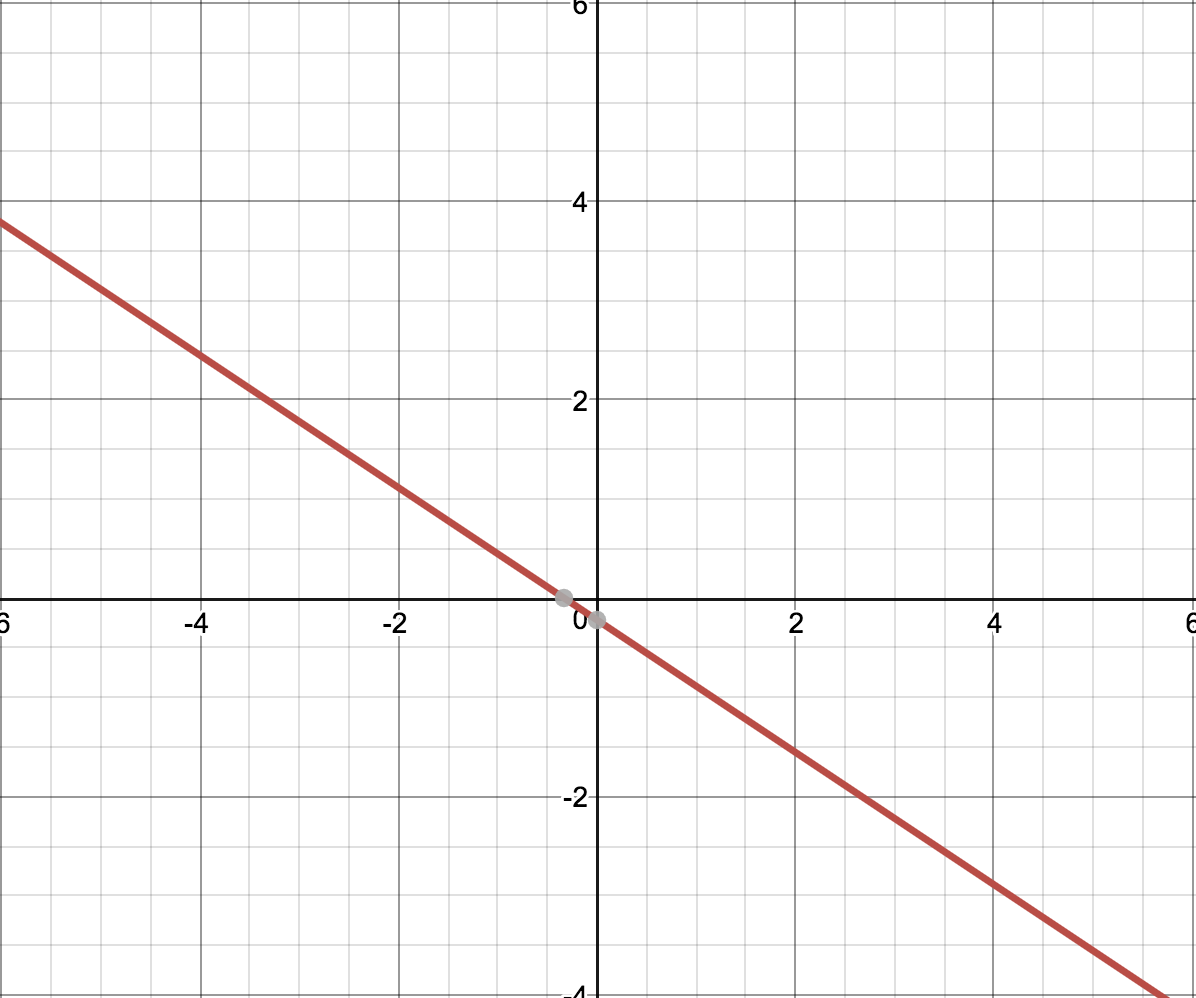
\includegraphics[width=0.5\textwidth]{c0.png}
        \caption{c = 0}
    \end{center}
\end{figure}
\begin{figure}[h!]
    \begin{center}
        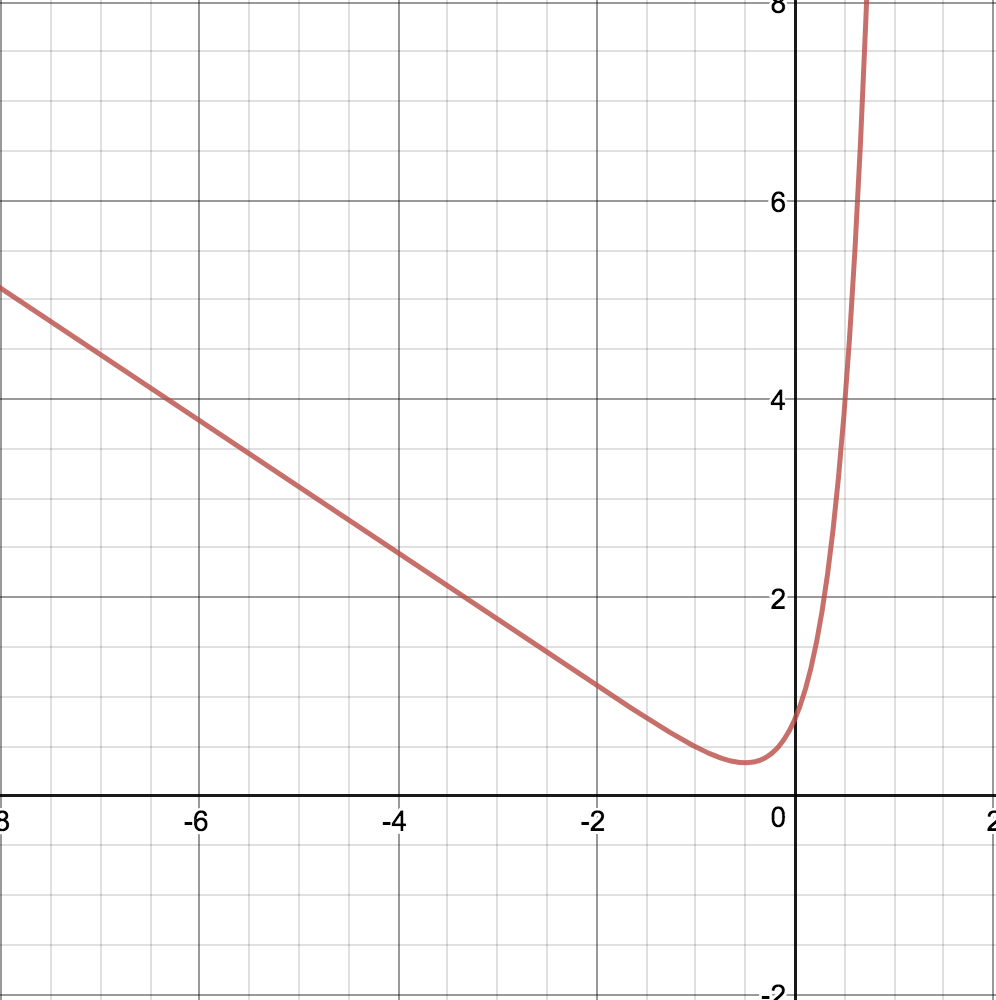
\includegraphics[width=0.5\textwidth]{c1.png}
        \caption{c = 1}
    \end{center}
\end{figure}

\begin{figure}[h!]
    \begin{center}
        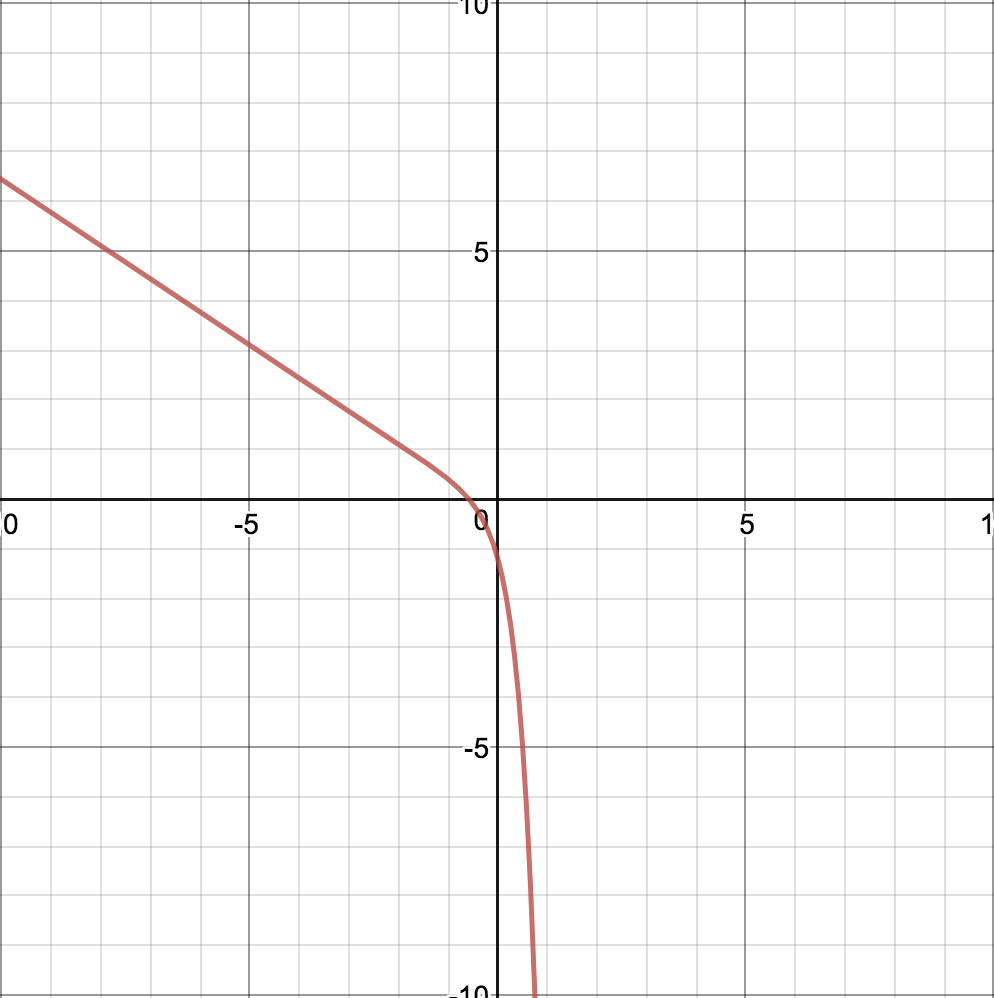
\includegraphics[width=0.5\textwidth]{c-1.png}
        \caption{c = -1}
    \end{center}
\end{figure}
\vspace{5000mm}
\clearpage
\newpage

\begin{center}
    {\LARGE 14th September Part 1}\\
\end{center}
\setcounter{subsection}{1}
\subsection{Linear ODE Revisited}
Consider $$\frac{dy}{dx} = p(x)y + q(x)$$
$$\frac{dy}{dx} - p(x)y = q(x) \;\;\;\;\;\;\;\;\;\;\;\text{Solution Set } S$$
$$\frac{dy}{dx} - p(x)y = 0 \;\;\;\;\;\;\;\;\;\;\;\text{Solution Set } \widetilde{S}$$

\textbf{Lemma 1:} If $y_1, y_2\; \epsilon\; \widetilde{S}$ then $c_1y_1 + c_2y_2\; \epsilon\; \widetilde{S}$, $c_1,\; c_2 \epsilon \R$ \\
\textit{Proof:} We know $\frac{dy}{dx} - p(x)y_1 = 0$ and $\frac{dy}{dx} - p(x)y_2 = 0$, what about $\frac{d}{dx}(c_1y_1 + c_2y_2) -p(x)(c_1y_1 + c_2y_2)$ On simplifying the last equation we get it's equal to zero \\\\
\textbf{Lemma 2:} Let $z_1,\;z_2\;\epsilon S$ then  $z_1,\;z_2\;\epsilon \widetilde{S}$\\
\textit{Proof:} We know $\frac{dz_1}{dy} - p(x)z_1 = q(x)$ and $\frac{dz_2}{dy} - p(x)z_2 = q(x)$, what about $\frac{d}{dx}(z_1-z_2) -p(x)(z_1-z_2) = 0$ On simplifying the last equation we get it's equal to zero \\\\
\textbf{Lemma 3:} Let $y_p\; \epsilon\; S$ (a particular solution), then $S\; =\; \{y+y_p:\; y\; \epsilon\; \widetilde{S}\}$
\textit{Eg: } $\frac{dy}{dx} -3y = 3x$
Consider  $\frac{dy}{dx} -3y = 0$, One solution is $y\equiv 0$ otherwise $\int\frac{dy}{y} = \int3dx$
$$\implies ln|y| = 3x + c \implies y = De^{3x}\;\;\;\;\;\;\;\; D \epsilon \R$$ Solution set of the associated homogeneous ODE is $\{De^3x: D\; \epsilon\; \R\}$
We need a $y_p$ - a special solution of the DE. We will guess this one. Let $$y_p = ax+b$$, $a$ and $b$ to be found.
$$\frac{dy_p}{dx} - 3y_p \equiv 2x \implies a -3(ax + b) \equiv 2x \implies a-3b - 3ax \equiv 2x$$
Comparing coefficients:
$$-3a = 2 \implies a = \frac{-2}{3}$$
$$a = 3b \implies b = \frac{-2}{9}$$
Thus $y_p = -\frac{2}{3}x - \frac{2}{9}$ and the complete solution set is $\{-\frac{2}{3}x - \frac{2}{9} + De^3x: D\; \epsilon\; \R\}$
\pagebreak
\subsection{Initial Value Problems}
When we solve a first order ODE we do not get a single function. We actually obtain a one parameter ($c$ - int constant) family of functions.\\
Often in practice we are provided with some extra information which allows us to choose one and only one of this family $i.e.$ the unique solution.\\
Often we have $x = x(t)$ and conditions at $t = 0$ and so the condition(s) of are referred to as initial condition.
The differential equation along with the initial condition together form an initial value problem

\begin{center}
    {\LARGE 14th September Part 2}\\
\end{center}

\paragraph{Aside Differentials}
$dx$ change in $x$, $dy$ change in $y$, leads to $dz$ change in $z$
$$z = H(x,y)$$
$$dz = \frac{\partial H}{\partial x}dx + \frac{\partial H}{\partial y} dy$$
But if we're on $z =\;\;\; constant \implies dz = 0 \implies z = c = H(x,\;y)$
$$0 = \frac{\partial H}{\partial x}dx + \frac{\partial H}{\partial y} dy \text{ [         implicit equation for } y]$$ and we can do something called implicit differentiation
$$\frac{\partial H}{\partial x} + \frac{\partial H}{\partial y} \frac{dy}{dx} = 0$$


\subsection{Exact $1^{st}$ order ODEs}
Suppose we have our $1^{st}$ order ODE $$\frac{dy}{dx} = F(x,y)$$. When we have to solve the ODE, we can always express the answer in the form $$G(x,y) = k$$ where k is a constant.

Our solution from earlier becomes: $$G(x,y) = \frac{y + \frac{2}{3}x + \frac{2}{9}}{e^{3x}}$$

If we differentiate this expression:
$$\frac{\partial G}{\partial x} + \frac{\partial G}{\partial y}\frac{dy}{dx} = 0$$
$$\implies \frac{dy}{dx} = -\frac{\frac{\partial G}{\partial x}}{ \frac{\partial G}{\partial y}}$$

Comparing the two $$\frac{dy}{dx} = F(x,y)$$ and $$\implies \frac{dy}{dx} = -\frac{\frac{\partial G}{\partial x}}{ \frac{\partial G}{\partial y}}$$

We must have, $$-\frac{\frac{\partial G}{\partial x}}{ \frac{\partial G}{\partial y}} = F(x,y)$$

There is some choice here:
$$\frac{\partial G}{\partial x} = m(x,y)F(x,y)$$
$$\frac{\partial G}{\partial y} = -m(x,y)$$
If we can find a $G(x,y)$ with $\frac{\partial G}{\partial x} = m(x,y)F(x,y)$ and
$\frac{\partial G}{\partial y} = -m(x,y)$. Then the solution is $G(x,y) = A$.

In practice we consider $\frac{dy}{dx} = F(x,y)$ is when teh function $F(x,y) = \frac{-M(x,y)}{N(x,y)}$, which we re-write as: $$M(x,y)dx + N(x,y)dy = 0$$
We want a solution of the following form $G(x,y) = c$
$$\frac{\partial G}{\partial x}dx + \frac{\partial G}{\partial y} dy = 0$$
We need         $$\frac{\partial G}{\partial x} = M(x,y)$$ and $$\frac{\partial G}{\partial y} = N(x,y)$$
\textit{How do we know whether these partial differential equations can be solved?}
If
$$\frac{\partial^2G}{\partial x \partial y} = \frac{\partial^2G}{\partial y \partial x}$$
Extending the earlier equations:
$$\frac{\partial }{\partial y}\frac{\partial G}{\partial x} = \frac{\partial M(x,y)}{\partial y} \equiv \frac{\partial }{\partial x}\frac{\partial G}{\partial y} = \frac{N(x,y)}{\partial x}$$

Given the ODE $mdx + Ndy = 0$ we say that the equation is exact to mean that the condition above is satisfied $\frac{N(x,y)}{\partial x} = \frac{\partial M(x,y)}{\partial y}$

\textit{Eg:}
$$
\frac{dy}{dx} = \frac{-1}{\frac{-(6y^2-x^2+3}{3x^2-3xy+2}}
$$
We re-write that as: $(3x^2-3xy+2)dx + (6y^2-x^2+3)dy = 0$\\
Is it possible that $\frac{\partial G}{\partial x} = 3x^2-2xy + 2 = M$ and $\frac{\partial G}{\partial y} = 6y^2 -x^2 + 3 = N$\\
We can solve this if $\frac{\partial^2G}{\partial x \partial y} = \frac{\partial^2G}{\partial y \partial x}$\\
$\frac{\partial M}{\partial y} = -2x$ and $\frac{\partial N}{\partial x} = -2x$
There is a solution, since this DE is exact\\\\
We want a function $G$ which $\frac{\partial G}{\partial x} = 3x^2 + 2xy + 2$
A solution is $G(x,y) = x^3 -x^2y + 2x$\\The most general solution is $G(x,y) = x^3 -x^2y + 2x + A(y)$ where $A(y)$ is a function of y\\\\
We also need $G$ to satisfy $\frac{\partial G}{\partial y} = 6y^2 -x^2 + 3$\\
A solution is $G = 2y^3 -x^2y + 3y$.\\ The most general solution is $G = 2y^3 -x^2y + 3y + B(x)$ where $B(x)$ for some function $B(x)$\\\\
Thus, the general solution of the DE is: $G(x,y) = x^3 + 2y^3 - x^2y + 2x + 3y + c$

\newpage

\begin{center}
    {\LARGE 18th September}\\
\end{center}
Last time we had the solution $G(x,y) = x^3 + 2y^3 - x^2y + 2x + 3y + k$\\
Solution is $G=c$, but we don't want two constants so we have to choose either of these:

$x^3 + 2y^3 - x^2y + 2x + 3y + k = 0$ or $x^3 + 2y^3 - x^2y + 2x + 3y = c$

Instead of remembering formulas remember:

$Mdx + Ndy = 0$ and that our solution for that is $\frac{\partial G}{\partial x}dx + \frac{\partial G}{\partial y}dy = 0$ and thus, $M=\frac{\partial G}{\partial x}$ and $N = \frac{\partial G}{\partial y}$.

And for a nice function $f$
$$\frac{\partial^2G}{\partial x \partial y} = \frac{\partial^2G}{\partial y \partial x} \implies \frac{\partial M}{\partial y} = \frac{\partial N}{\partial x}\;\;\;\;\;\;\;\;\;\;\;\; \text{Clairaut's theorem on equality of mixed partials}$$

\subsubsection{Why could the Clairaut's theorem on equality of mixed partials fail for a G}
$$xe^{xy} = c$$
Differentiating,
$$(e^{xy}+xye^{xy})dx + x^2e^{xy}dy = 0 \implies \frac{dy}{dx} = -\frac{e^{xy} + xye^{xy}}{x^2e^{xy}} \;\;\;\;\;\;\; xy \neq 0$$
And since $e^{xy} \neq 0$ then can we not factor it out of the equation
$$(1+xy)dx + x^2dy = 0$$
Now the question being whether this is exact?
Let $$M = 1+xy\;\;\;\;\;\;\;\;\;\;\; N = x^2$$
$$\;\;\frac{\partial M}{\partial y} = x\;\;\;\;\;\;\;\;\;\;\;\;\;\;\;\;\; \frac{\partial N}{\partial x} = 2x$$
This means that the equation earlier is not exact since there are not exactly the same functions.

Now we are in a situation that we need to find the missing function, and need to find what it is. It's called the Integration factor method
\subsection{Integration Factors}
Suppose we have to find a first order ODE that is not exact.\\
How de we proceed?\\
Solution: We multiply the ODE by an unknown function $I(x,y)$, called an integration factor. We try to make the new ODE exact
$$\text{i.e.} \;\;\; Mdx + Ndy = 0$$
And $M_y \not\equiv N_x \;\;\;\; \text{which is not exact, and we remedy by multiplying with I} \implies MIdx + NIdy = 0$\\
We want this to be exact  $(MI)_y \equiv (NI)_x$, which now imposes a restriction on $I$\\\\
Sadly we started from an ODE, but we moved to a PDE i.e. we are in a bigger mess now. Differentiating:
$$I\frac{\partial M}{\partial y} + M\frac{\partial I}{\partial y} \equiv I\frac{\partial N}{\partial x} + N\frac{\partial I}{\partial x} \;\;\;\;\;\;\;\;\;\;\;\; (**)$$
This is very hard to solve in general, however there are two special cases:\\
\textbf{Case 1:}
$I(x,y) = I(x)$ The PDE $(**)$ becomes
$$I\frac{\partial M}{\partial y} \equiv I\frac{\partial N}{\partial x} + N\frac{dI}{dx}$$

Collect all the terms in $I$ together,
$$\frac{1}{I}\frac{dI}{dx} = \frac{1}{N}(\frac{\partial M}{\partial y} - \frac{\partial N}{\partial x})$$
Since the LHS in the left, is just a function of $x$ only, then the RIHS must also be a function of $x$ only.\\
The RHS involves terms from the ODE, and we now have a test for an integration factor of the form $I = I(x)$

\textit{Eg:} = $\frac{dy}{dx} = -\frac{1+xy}{x^2}$, given $x^2 \neq 0$
$$(1+xy)dx + (x^2)dy$$
$$\implies M = 1+xy \implies M_y = x$$
$$\implies N = x^2 \implies N_x = 2x$$
Thus, $x \not\equiv 2x$, i.e. they are not identical, but they can be equal at $x = 0$
We examine $\frac{M_y - N_x}{N} = \frac{x-2x}{x^2} = -\frac{1}{x}$\\
Since is this a function of $x$ only,
\begin{itemize}
    \item There will be an integration factor for the DE of the form $I(x,y) = I(x)$
    \item $\frac{dlnI}{dx} = -\frac{1}{x}$, integration $ln(I) = ln|\frac{1}{x}|$ and one solution is $I(x) = x^{-1}$
\end{itemize}
Solution: $(1+xy)dx + x^2dy = 0$, multiplying by $I(x)$ we get $$(x^{-1} +y)dx + xdy = 0$$
Find $G(x,y)$ such that $G_x = x^{-1} + y \implies ln|x| + xy + H(y) = G$
and $G_y = x \implies xy + H(x) = G$\\
Therefore $G(x,y) = xy + ln|x|$ and the solution becomes: $G(x,y) = xy + ln|x| = c$\\

\begin{center}
    {\LARGE 21st September Part 1}\\
\end{center}
\textbf{Case 2:}  $I = I(y)$ and $I_x = 0$
$$I_yM + IM_y -IN_x = 0$$
$$\frac{dI}{dy}\frac{1}{I} = \frac{N_x-M_y}{M}$$
The LHS is only a function of $y$ then the RHS must also be a function of $y$\\
We need a combination $\frac{M_y-N_x}{-M}$ to be a function of only $y$. In this, we will be able to obtain $I(y)$ i.e. an integration factor which is a function of only $y$\\
$$\frac{dy}{dx} = \frac{-y^2}{1+xy} \implies y^2dx + (1+xy)dy = 0$$
$M = y^2$ and $N=1+xy$\\
$M_y = 2y$ and $N_x = y$, so this DE is not exact\\
We multiply by $I(x,y)$ to get $$Iy^2dx + I(1+xy)dy = 0 \;\;\;\;\;\;\; (1)$$
Consider $I = I(x)$
$(Iy^2)_y = I2y$ and $(I(1+xy))_x =  \frac{dI}{dx}(1+xy) + I_y$\\
If $(Iy^2)_y = (I(1+xy))_x$ then $2yI = \frac{dI}{dx}(1+xy) + I_y$
$\implies \frac{dI}{dy}\frac{1}{I} = \frac{y}{1+xy}$, in which sadly RHS is not just a function of $x$ while LHS is\\
Now considering, $I = I(y)$
$(Iy^2)_y = \frac{dI}{dy}y^2 + 2yI$ and $(I(1+xy))_x = I_y $\\
If we equate these, $y^2\frac{dI}{dy} + 2yI = I_y \Longleftrightarrow y^2\frac{dI}{dy} + yI$\\
Assuming $y \not \equiv 0$,
$$\frac{dI}{dy}\frac{1}{I} = -\frac{1}{y}$$
Integrating we get,
$$ln|I| = -ln|y| \implies ln|I||y| = 0 \implies |Iy| = e^0 \implies Iy = \pm 1 \implies I = \frac{1}{y} \;\;\;\; \text{(Choosing the positive one only)}$$
$(1)$ becomes,
$$ydx + \frac{1+xy}{y}dy = 0$$
There exists a $G(x,y)$ such that
$G_x = y \implies G= xy + F(y)$ and $G_y = \frac{1}{y} + x \implies G = xy + ln|y| + H(x)$\\
Thus,
$$G = xy + ln|y| \;\;\;\;\; \text{and the Solution is } G = xy + ln|y| = c$$
\section{Second Order Linear ODEs}
$$a_2(x)\frac{d^2y}{dx^2} + a_1(x)\frac{dy}{dx} + a_0(x)y = f(x)$$
We will only deal with those equation when $a_2, a_1, a_0$ are all constants and not functions\\
We say that the DE has constant coefficients to mean that $a_2(x) = constant, a_1(x) = constant, a_0(x) = constant$\\
Dividing by $a_2(x)$, we get $$\frac{d^2y}{dx^2} + p\frac{dy}{dx} + qy = f(x)$$

$$\frac{d^2y}{dx^2} + p\frac{dy}{dx} + qy = f(x) \;\;\;\;\;\;\; \text{Solution set } S$$
$$\frac{d^2y}{dx^2} + p\frac{dy}{dx} + qy = 0 \;\;\;\;\;\;\; \text{Solution set } \tilde{S}$$
The second equation above is the associated homogeneous DE

\textbf{Lemma 1:} $\tilde{S}$ is a vector subspace of function space (It is a 2 dimensional)\\
\textbf{Lemma 2:} $z_1, z_2 \; \epsilon\; S$  then $z_1\; -\; z_2\; \epsilon\; \tilde{S} $\\
\textbf{Lemma 3:} $S = \{y_p + y: y\; \epsilon\; \tilde{S}\}$ where $y_p\; \epsilon\; S$\\

We begin by considering $\tilde{S}$, i.e. solve
$$\frac{d^2y}{dx^2} + p\frac{dy}{dx} + qy = 0$$

\newpage
\begin{center}
    {\LARGE 21st September Part 2}\\
\end{center}
Try to  $e^{mx}$ and adjust m to make this work\\
Putting $y = e^{mx}$ into the LHS of the DE with
$\frac{dy}{dx} = me^{mx}$ and $\frac{d^2y}{dx^2} = m^2e^{mx}$\\
We get, $m^2e^{mx} + pme^{mx} + qe^{mx} - (m^2 + pm + q)e^{mx}$
We want to get $0$ in RHS, thus
We need $(m^2 + pm + q)e^{mx} \equiv 0$\\
$e^{mx} \neq 0 \implies (m^2 + pm + q) = 0$\\
There are three cases:
\begin{itemize}[topsep=-10pt]
    \item Two real distinct roots $m_1, m_2$\\
    Two solutions $e^{m_1x}, e^{m_2x}$ which are two linearly independent solutions\\
    General solution: $y = Ae^{m_1x} + Be^{m_2x}$\\
    Solution set is $\{Ae^{m_1x} + Be^{m_2x}\} = span(\{e^{m_1x}, e^{m_2x}\})$
    \item Real equal roots $m_1 = m_2$; $y = e^{m_1x}$ is a solution\\
    This is bad luck (i.e. Conrad Resonance of Type 1)\\
    Another independent solution is $y_2 = xy_1 = xe^{m_1x}$\\
    General solution: $Ae^{m_1x} + Bxe^{m_1x}$\\
    Solution set is $\{Ae^{m_1x} + Bxe^{m_1x}\} = \{span(\{e^{m_1x}, xe^{m_1x}\})$
    \item Two complex roots
    $m_1 = \alpha + j\beta ,\;\; m_2 = \alpha - j\beta \;\;\;\;\;\;\; \alpha\; \epsilon\; \R,\;\;\;\; \beta\; \epsilon\; \R\; -\; \{0\}$\\
    $$y_1 = e^{m_1x} = e^{(\alpha + j\beta)x} = e^{\alpha x} e^{j\beta x} = e^{\alpha x} (cos\beta x + j sin \beta x)$$
    $$y_2 = e^{m_2x} = e^{(\alpha - j\beta)x} = e^{\alpha x} e^{-j\beta x} = e^{\alpha x} (cos\beta x - j sin \beta x)$$
    $$\text{sum/2: } e^{\alpha x}cos(\beta x) = y_1\;\;\;\;\;\;\; \text{This is real}$$
    $$\text{difference/(2j): } e^{\alpha x}sin(\beta x) = y_2\;\;\;\;\;\;\; \text{This is real too}$$\\
     General solution: $Ae^{\alpha x}cos(\beta x) + Be^{\alpha x}sin(\beta x)$\\
    Solution set is $\{Ae^{\alpha x}cos(\beta x) + Be^{\alpha x}sin(\beta x), \;\;\; A,\; B\; \epsilon\; \R\}$
\end{itemize}

\textbf{Note:} $Acos(\beta t) + B sin(\beta t) = Rcos(\beta t - \phi)$
then $R = \sqrt{A^2 + B^2}$ and $tan(\phi) = \frac{B}{A}$\\
\textit{Eg:} Solve
\begin{itemize}[topsep=-10pt]
    \item $y'' + 2y' -8y = 0$\\
    Try $e^{mx}$, we get $(m^2 + 2m - 8)e^{mx} = 0 \implies (m^2 + 2m - 8) = 0$ \\$\implies (m+4)(m-2) = 0 \implies m = -4, 2$\\
    The two linearly independent solutions are $y_1 = e^{-4x},\; y_2 = e^{2x}$
    \item $y'' - 10y' + 25y = 0$
    Try $e^{mx}$, we get $(m^2 -10m + 25)e^{mx} = 0 \implies (m^2 -10m + 25) = 0$ \\$\implies (m-5)(m-5) = 0 \implies m = 5$\\
    One solution is $y_1 = e^{5x}$. This is bad luck (i.e. Conrad Resonance of Type 1), and therefore the second solution is $y_2 = xe^{5x}$\\
    The two linearly independent solutions are $y_1 = e^{5x},\; y_2 = xe^{5x}$\\
    Solution set is $\{Ae^{5x} + Bxe^{5x},\; A,\; B\; \epsilon\; \R\}$\\
    Let us check $y_2: $, $y_2' = (1+5x)e^{5x}, y_2'' = (10 + 25x)e^{5x}$ \\
    Putting this back in the original differential equation results in zero
    \item $y'' - 2y' + 5y = 0$
    Try $e^{mx}$, we get $(m^2 - 2m + 5)e^{mx} = 0 \implies (m^2 - 2m + 5) = 0$ \\$ \implies m = 1 \pm 2j$\\
    We have

\end{itemize}
\newpage

\begin{center}
    {\LARGE 24th September}\\
\end{center}
Today we consider a particular solution of the inhomogeneous differential equation.
$$y'' + py' + qy = f(x)$$
We want $y_p$
\subsection{The method of undetermined coefficients}
The guiding principle is to choose something "like" $f(x)$


\begin{table}[h!]
\begin{tabular}{|l|l|}
\hline
\textbf{$f(x)$}                           & \textbf{Try for $y_p$}                   \\ \hline
Polynomial of order n            & Polynomial of order n           \\ \hline
Exponential $e^{\alpha x}$       & $ae^{\alpha x}$                 \\ \hline
$sin(\beta t)$ or $cos(\beta t)$ & $asin(\beta t) + bcos(\beta t)$ \\ \hline
Sums and/or products of above    & Sums and/or products of above   \\ \hline
\end{tabular}
\end{table}

\textit{Eg:} $y'' + 2y' - 8y = x^2 + 2x + 3$\\
When we solved the homogeneous equation $y'' + 2y' - 8y = 0$ the solution was $y = Ae^{2x} - Be^{-4x}$

Let $y_p = ax^2 + bx + x \implies$ $y_p' = 2ax + b$ and $y_p'' = 2a$
Putting this into the LHS of the equation:
$$2a + 4ax + 2b - 8ax^2 -8bx - 8c$$ while the RHS is $x^2 + 2x + 3$\\
For $x^2 \implies 8a = 1 \implies a = -\frac{1}{8}$\\
For $x \implies 4a - 8b = 2 \implies b = \frac{4a - 2}{8} \implies b = -\frac{5}{16}$\\
For constants$ \implies 2a + 2b - 8c = 3 \implies c = \frac{2a + 2b - 3}{8} \implies c = -\frac{31}{64}$\\
$\implies y_p = -\frac{1}{8}x^2 -\frac{5}{16}x -\frac{31}{64}$, with the general solution being $y = y_p + Ae^{2x} + Be^{-4x}$\\

Going to be on the test?\\
\textit{Eg:} $y'' + 2y' - 8y = xe^{3x}$\\
Try $y_p = (A+Bx)e^{3x}$, write down the most general polynomial of the RHS\\
$y_p' = [3A + 3Bx + + B]e^{3x}$ and $y_p'' = [9A + 9Bx + + 3B + 3B]e^{3x}$\\
Put these terms into the LHS of the equation to get:\\
$(9A + 6B + 9Bx + 6A + 2B + 6Bx -8a -8Bx)e^{3x} = ((7A + 8B) + (7B)x)e^{3x}$\\
We want to get $xe^{3x}$
Comparing coefficients:\\
For $xe^{3x} \implies 7B = 1 \implies B = \frac{1}{7}$\\
For $e^{3x} \implies 7A + 8B = 0 \implies A = -\frac{8}{49}$\\
$y_p = (-\frac{8}{49} + \frac{x}{7})e^{3x}$ with the general solution being $y = y_p + Ce^{2x} + De^{-4x}$, $C,\;D\;\epsilon \R$

\textit{Eg:} $y'' + 2y' - 8y = sin(2x)$\\
Try $y_p = asin2x + bcos2x$, $y_p' = 2acos2x -2bsin2x$ and $y_p'' = -4asin2x - 4bcos2x$\\

We put $y_p$ into the LHS of the DE:\\
$-4y_p + 2(acos2x - 2bsin2x) -8y_p = 4acos2x - 4bsin2x -12asin2x - 12bcos2x$\\
We get $(-4b-12a)sin2x + (4a-12b)cos2x$ which we want to equal $sin(2x)$
Comparing coefficients:\\
For $cos2x \implies 4a-12b = 0 \implies a = 3b$\\
For $sin2x \implies -4b-12a = 1 \implies a(-12 - \frac{4}{3}) = 1 \implies a = -\frac{3}{40}$ and $b = -\frac{1}{40}$\\

$y_p = -\frac{3}{40}sin2x + -\frac{1}{40}cos(2x)$ with the general solution being $y = y_p + Ce^{2x} + De^{-4x}$, $C,\;D\;\epsilon \R$

\textit{Eg:} $y'' + 2y' - 8y = e^{2x}$\\
Try $y_p = ae^{2x}$
We put $y_p$ into the LHS of the DE:\\
LHS becomes zero, because it is already of the homogeneous solution.
We know that this will give zero, i.e. we have bad luck (i.e. Conrad Resonance of Type 2)\\
Instead we try:
$y_p = x(ae^{2x}) \implies y_p' = a(2x+1)e^{2x}$ and $y_p'' = a(4x+2+2)e^{2x}$\\
Putting this in the LHS of the DE we get $a(4x + 4 + 4x + 2 - 8x)e^{2x} = 6ae^{2x}$\\
We want this to be equal to RHS, we need $6a = 1 \implies a = \frac{1}{6}$



\textit{Eg:} $y'' - 10y' +25y = x^2e^{5x}$\\
When we solved the homogeneous equation $y'' - 10y' +25y = 0$ the solution was $y = Ae^{5x} - Bxe^{5x}$\\
What do we try: $y_p = (ax^2+bx+c)e^{5x}$, this way the terms with $b$ and $c$ are part of the homogeneous and they will get cancelled i.e. we have bad luck (i.e. Conrad Resonance of Type 3)\\
We use $x^2$ because it is over 2
Thus we have to try: $y_p = x^2(ax^2+bx+c)e^{5x}$

\newpage

\begin{center}
    {\LARGE 25th September}\\
\end{center}
\subsection{Initial Conditions}
Since the DE is $2^{nd}$ order we need 2 peices of information for a particular DE
\begin{enumerate}
    \item Initial Values/conditions\\
    $x(0) = x_0$ and $\frac{dx}{dt}|_{t = 0} = V_0$
    \item Boundary Value Problem\\
    $x(0) = x_0$ and $x(T) = x_1$
    \item Mixed conditions\\
    Either $x(0) = x_0$ and $\frac{dx}{dt}|_{t = T} = V_t$ or $x(T) = x_1$ and $\frac{dx}{dt}|_{t = 0} = V_0$
\end{enumerate}
\textit{Eg:} $y'' +2y' -8y = sin(2x)$ when $y(0) = 0 , y'(0) = 0$\\
We already solved this earlier, so using given information:
$y(0) = a + b - \frac{1}{40}$ and $y'(0) = 2a - 4b -6/40 \implies a = \frac{1}{60}, b = \frac{1}{120}$
\subsubsection{The Oscillator DE}
$\ddot{x} + 2\lambda\dot(x) + \omega_0^2x = F(t)$ i.e. $\frac{d^2x}{dt^2} + 2\lambda \frac{dx}{dt} + \omega_0^2x = F(t)$
\subsubsection{LCR Circuits}
Using Kirchoff's Law's\\
$IR + \frac{Q}{C} + L\frac{dI}{dt} = V(t)$\\
Since we know $I = \frac{dQ}{dt} \implies \frac{d^2Q}{dt^2} + \frac{R}{L}\frac{dQ}{dt} + \frac{Q}{C\dot L} = \frac{V(t)}{L}$
\subsubsection{Mass on Spring}
Spring constant k \\ Hooke's Law $F = -kx$\\ Air resistance for low velocity $\approx \alpha \frac{dx}{dt}$\\
$\frac{d}{dt}(mv) = mg -kx -\alpha \frac{dx}{dt}$
\newpage


\begin{center}
    {\LARGE 27th September}\\
\end{center}
\textit{Eg:} C-R circuit\\
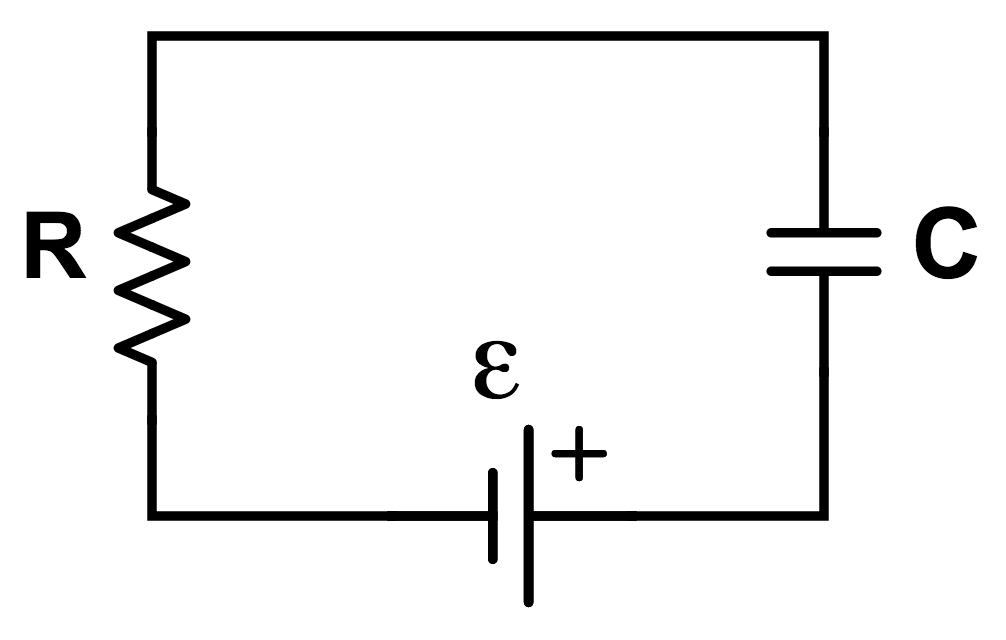
\includegraphics[width=0.5\textwidth]{RC.png}\\
Applying Kitchoff's Law: $IR + \frac{Q}{C} = V(t)$ but $I = \frac{dQ}{dt}$\\
Linear for V = V(t), separable if $V(t) = K$\\
Multiply by integration factor $J(t)$ \\
$$J\frac{dQ}{dt} + \frac{JQ}{RC} = J\frac{V}{R}$$
We insist that the LHS is $\frac{d}{dt}(J(t)Q(t)) \implies \frac{dJ}{dt}Q + J\frac{dQ}{dt}$\\
We need: $\frac{dJ}{dt}Q = \frac{JQ}{RC}$, and for $Q \not\equiv 0$ we have $\frac{dJ}{dt} = J\frac{1}{RC}$.\\
Solving for $J$ in the second equation we get $J = e^{\frac{t}{RC}}$\\
At this point we can rewrite teh original equation as:
$$\frac{d}{dt}(Qe^{\frac{t}{RC}}) = \frac{1}{R}e^{\frac{t}{RC}}V(t)$$
\begin{enumerate}
    \item Let $V(t) = V_0$ be a constant DC supply\\
    The DE is now
    $$\frac{d}{dt}(Qe^{\frac{t}{RC}}) = \frac{V_0}{R}e^{\frac{t}{RC}}$$
    Integrating:
    $$Qe^{\frac{t}{RC}} = \frac{V_0}{R}RCe^{\frac{t}{RC}} + K\;\;\;\;\;k \epsilon R$$
    $$Q = V_0C + Ke^{-\frac{t}{RC}}$$
    The steady state term is $V_0C$ with the transient term being $Ke^{-\frac{t}{RC}}$\\
    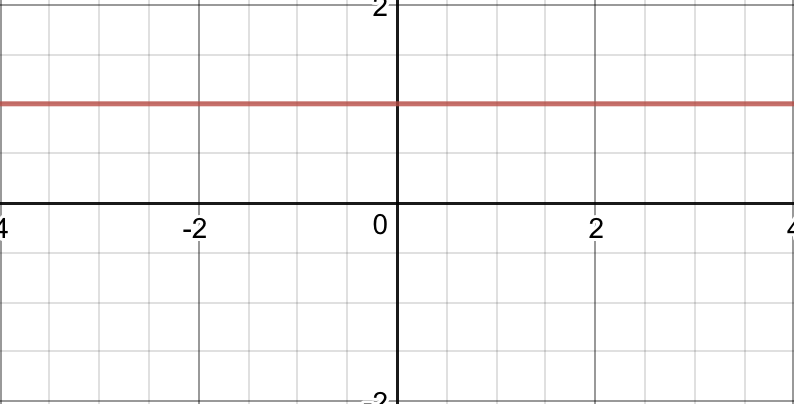
\includegraphics[width=0.5\textwidth]{constant.png}\\
    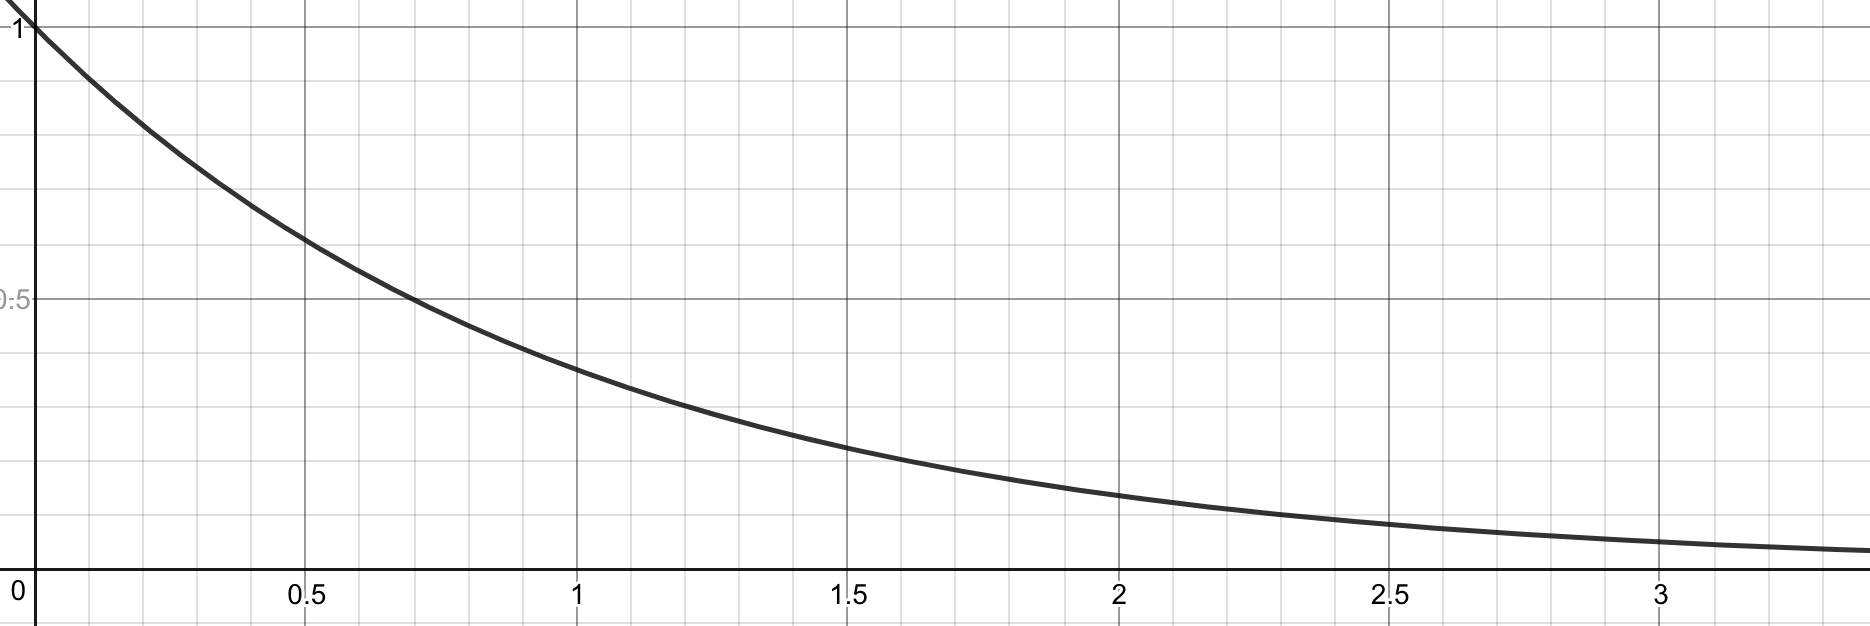
\includegraphics[width=0.5\textwidth]{etrc.png}\\
    $t = RC$, $RC$ is a time in seconds which provides us with a measure of how long the transient term is significant
    \item Let $V(t) = V_0sin(\omega t)$ a constant AC supply\\
    $$\frac{d}{dt}e^{\frac{t}{RC}}Q = e^{\frac{t}{RC}}\frac{V_0}{R}sin(\omega t)$$
    Integrating we get:
    $$Q = \frac{V_0C}{1+\omega^2R^2C^2} [-\omega RC cos(\omega t) + sin(\omega t)] + ke^{\frac{-t}{RC}}$$\\
    The first part is the steady state term, and other one dies away and is the transient part
\end{enumerate}
\newpage

\begin{center}
    {\LARGE 28th September}\\
\end{center}
\newgeometry{top=-10mm, bottom=4mm, left=10mm, right=10mm}
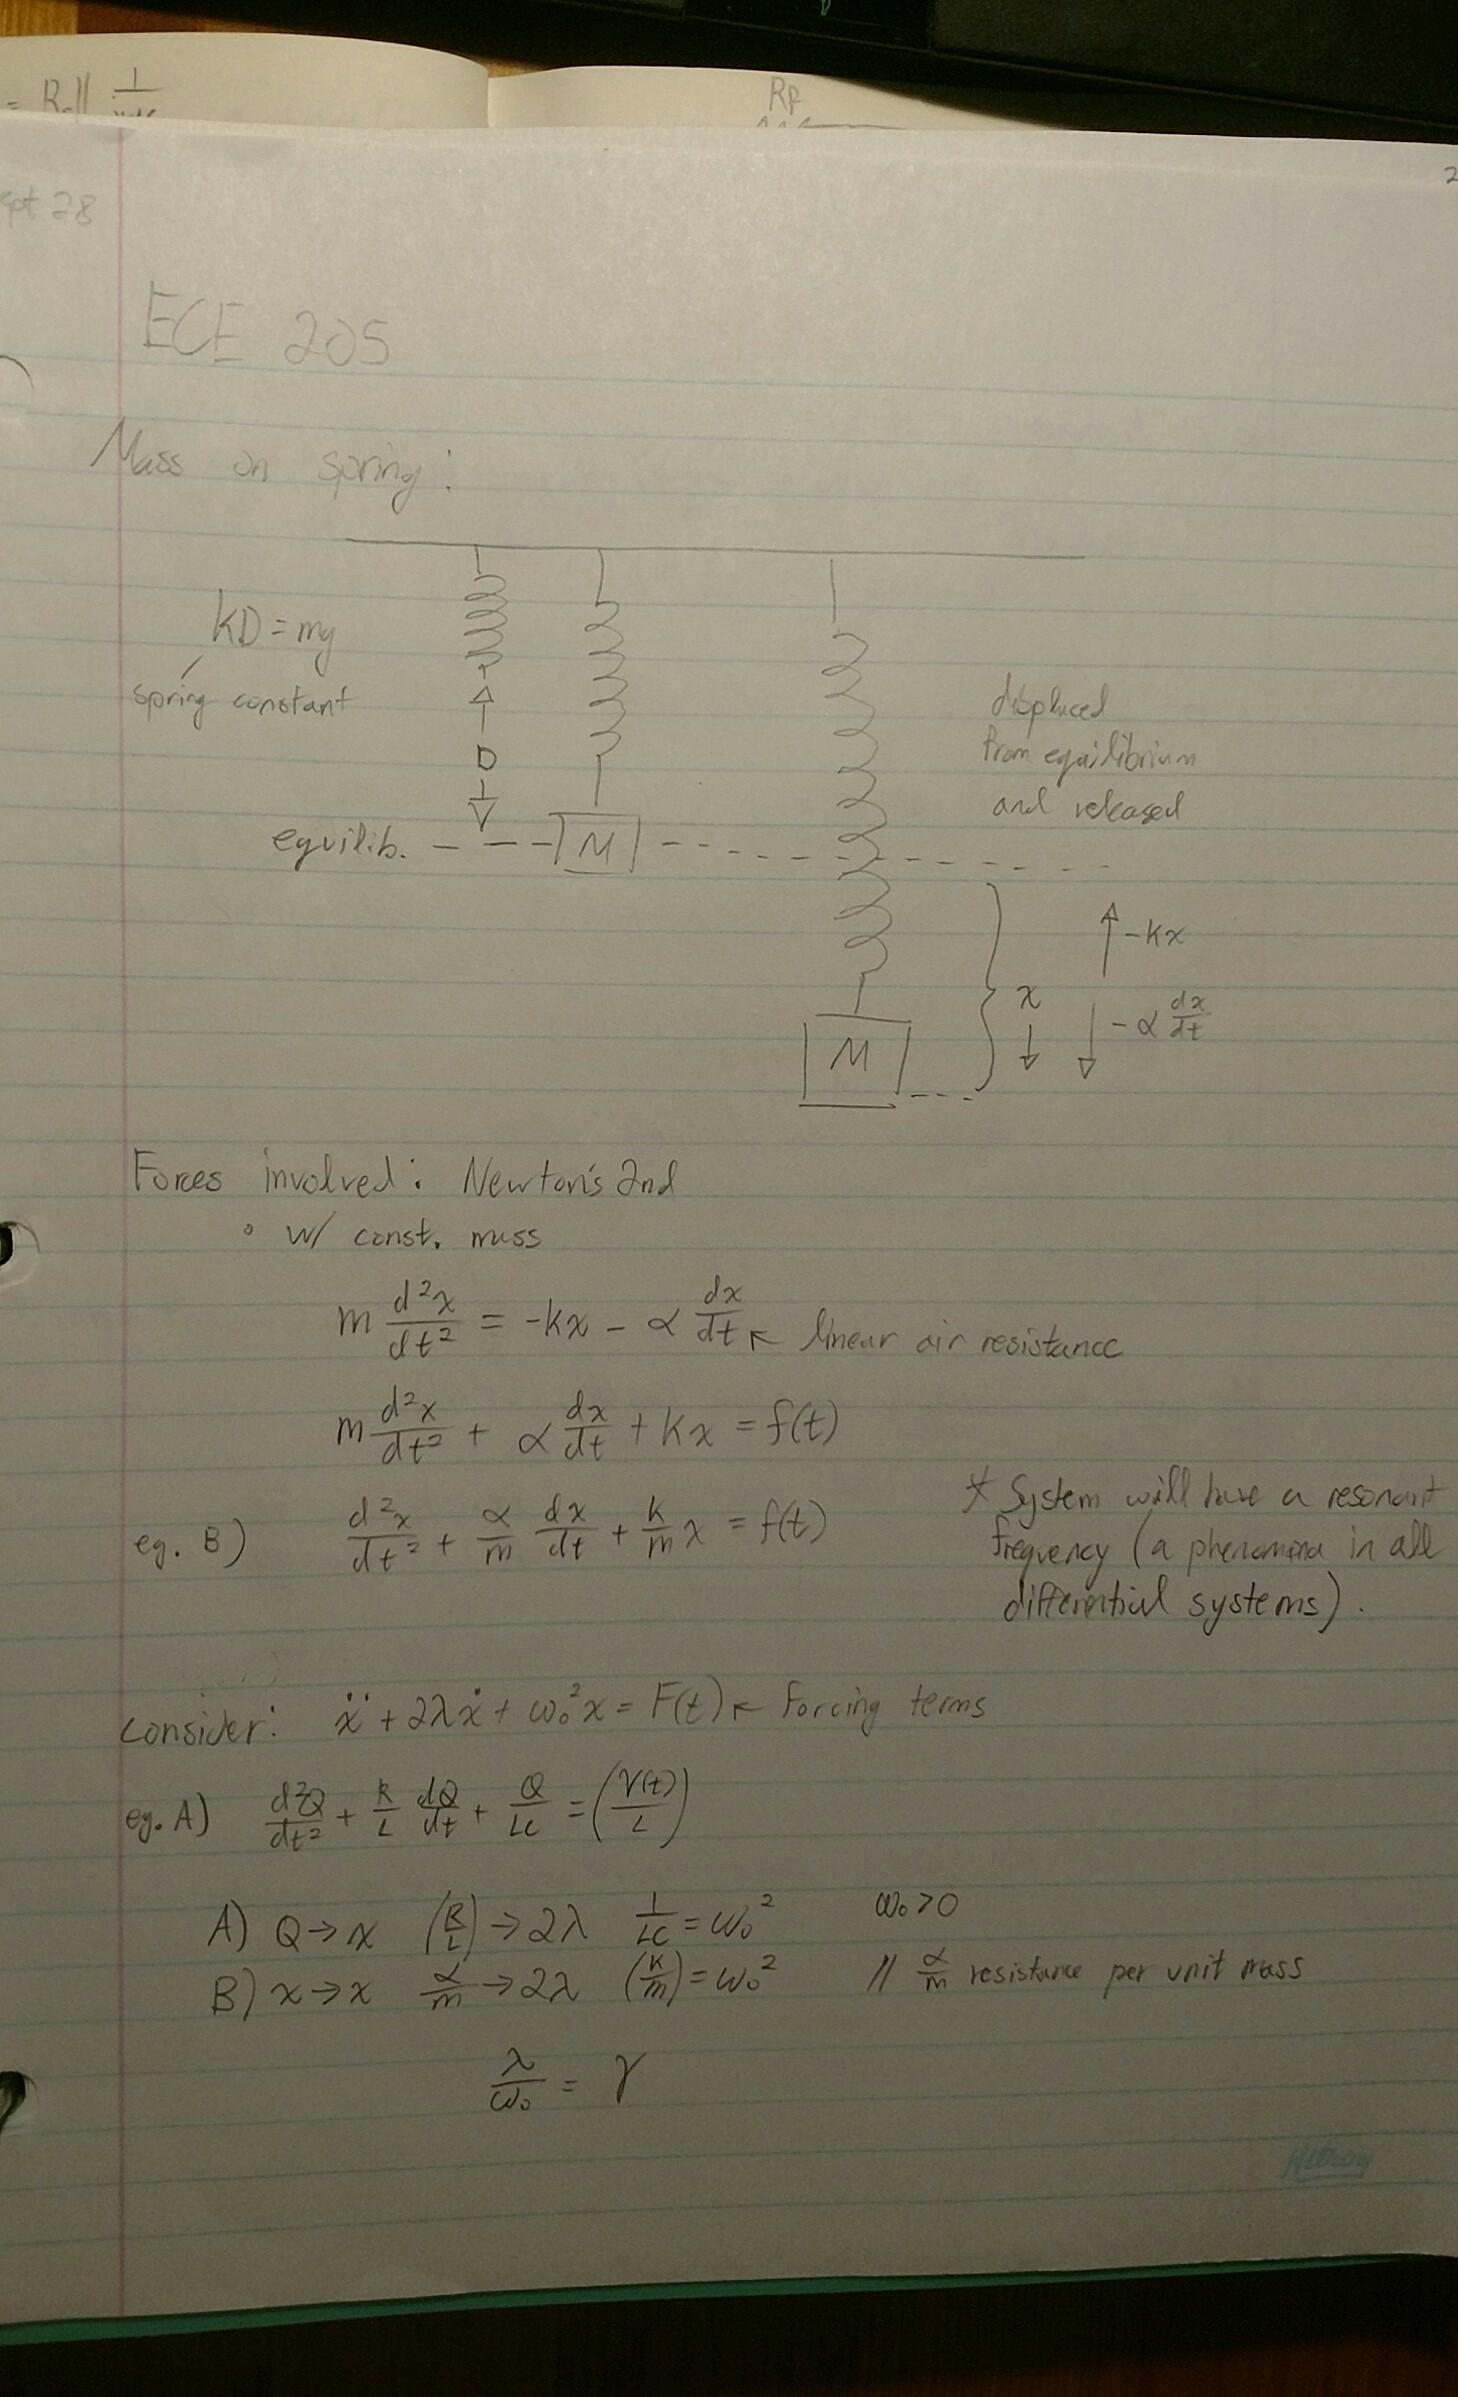
\includegraphics[width=\textwidth,height=\textheight,keepaspectratio]{friday/1.jpg}\\
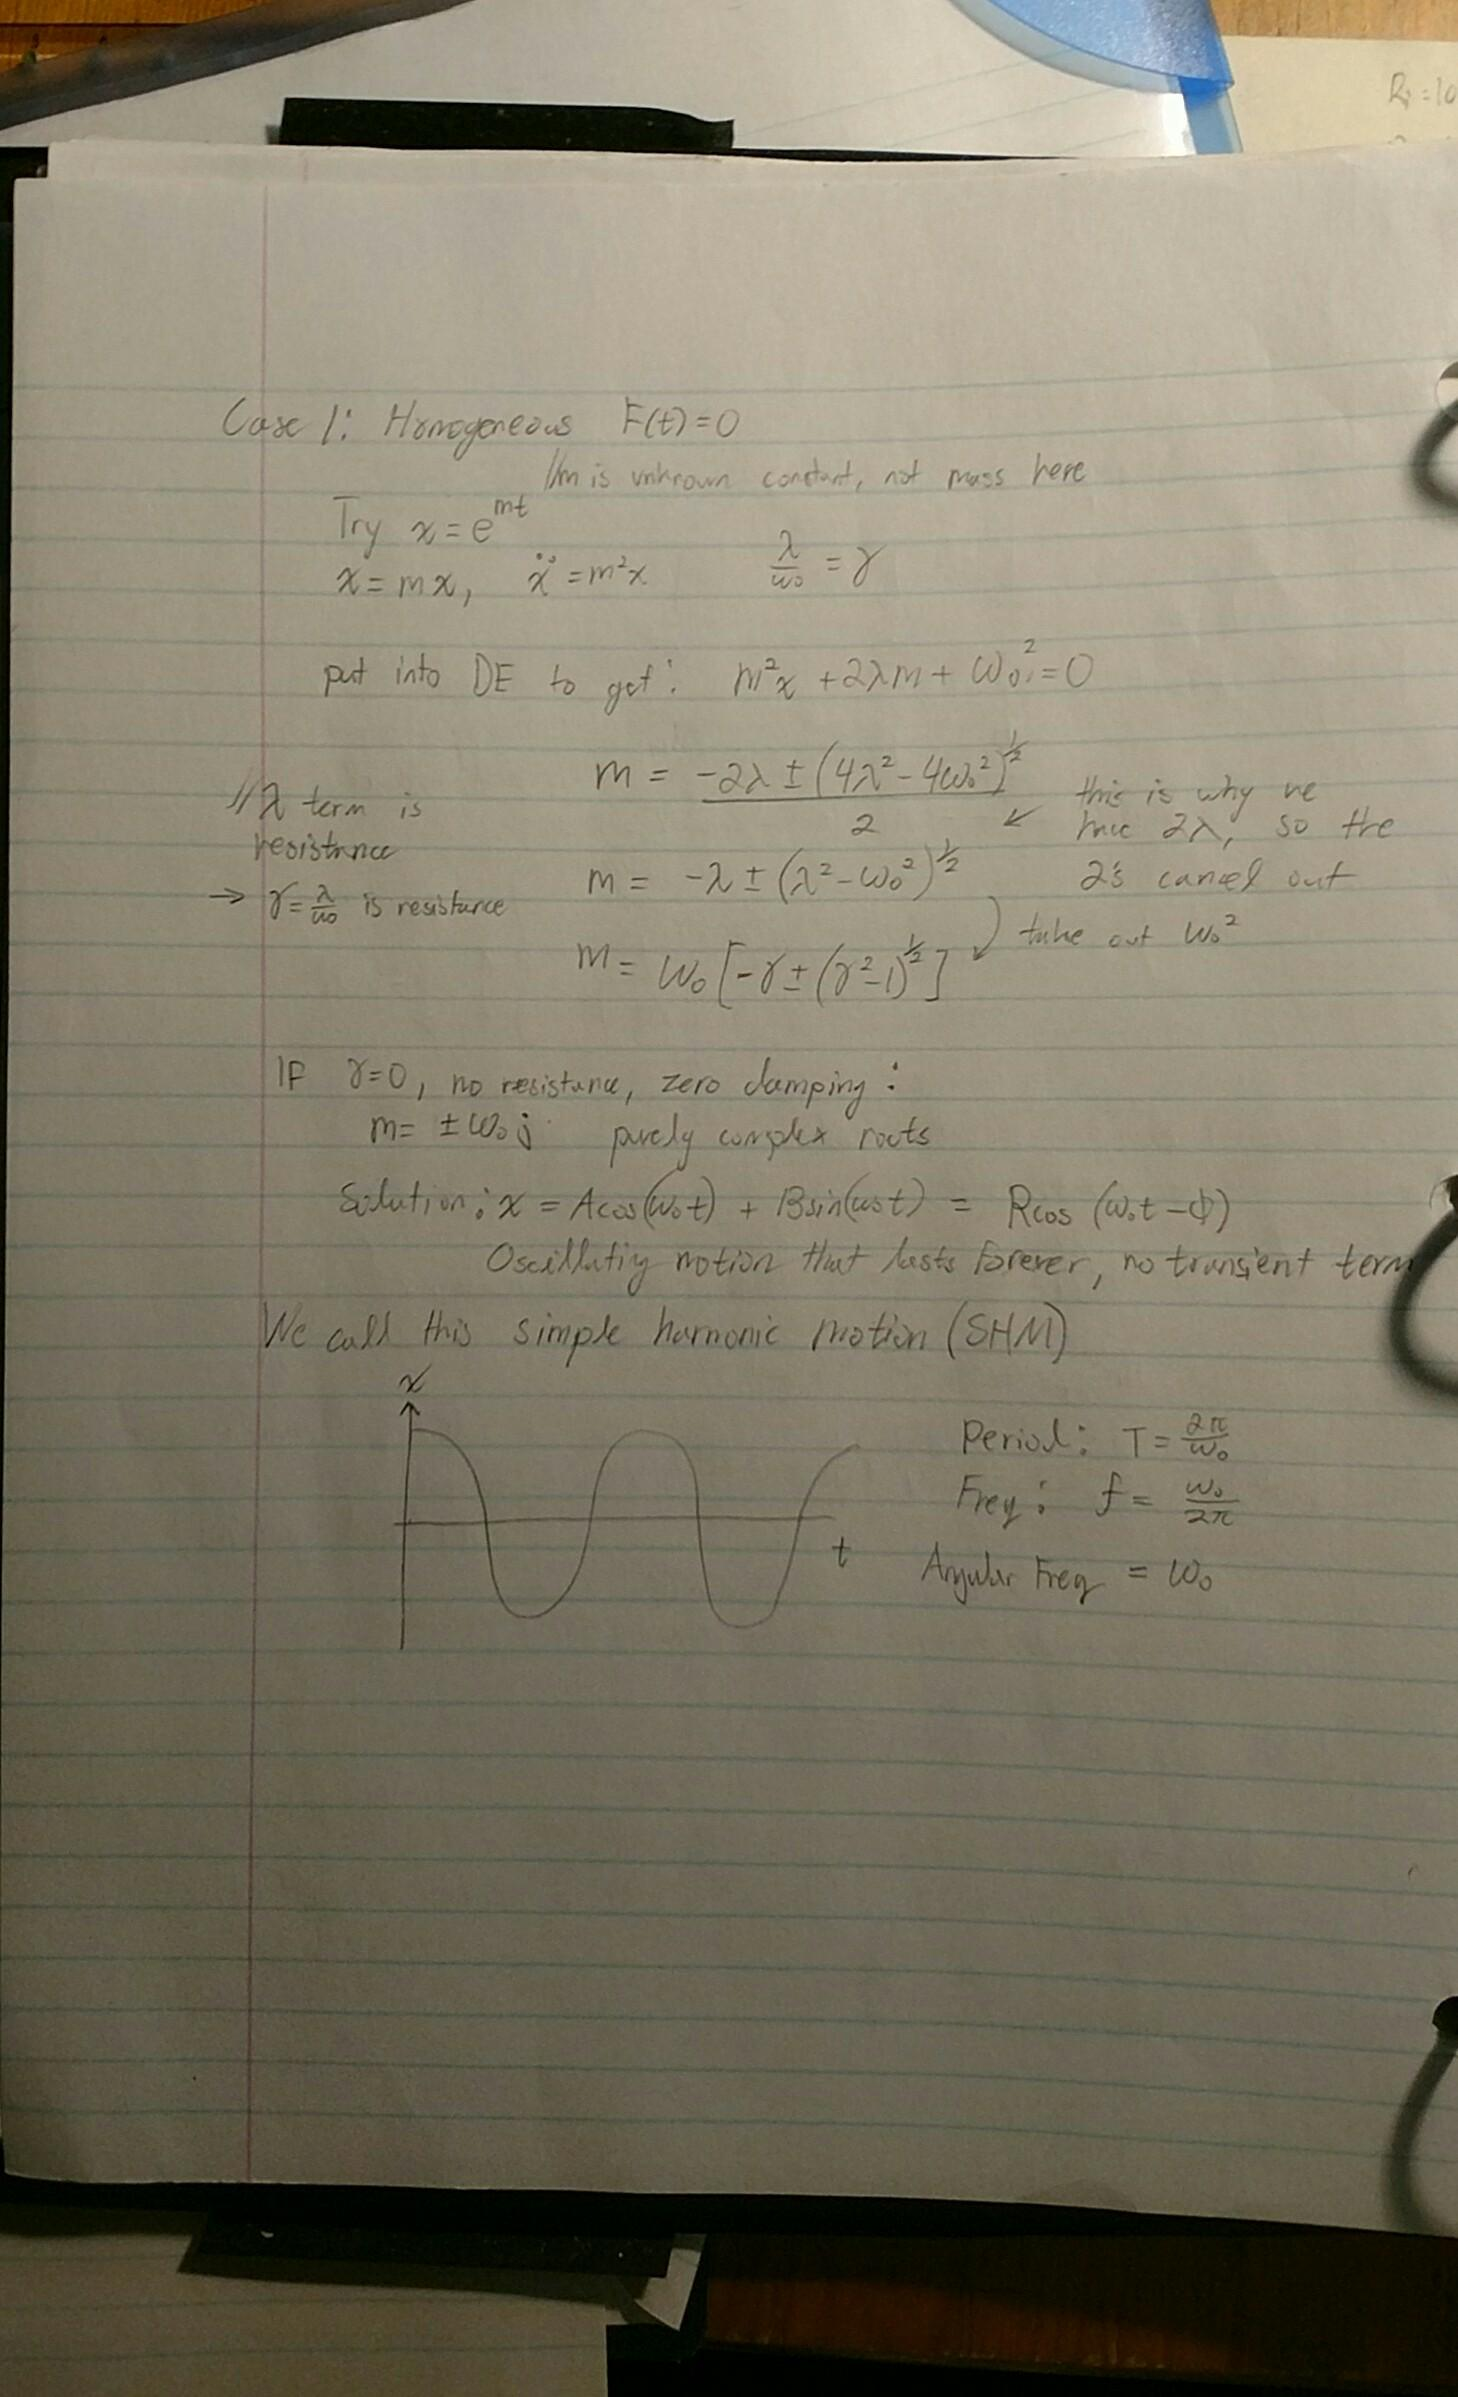
\includegraphics[width=\textwidth,height=\textheight,keepaspectratio]{friday/2.jpg}\\
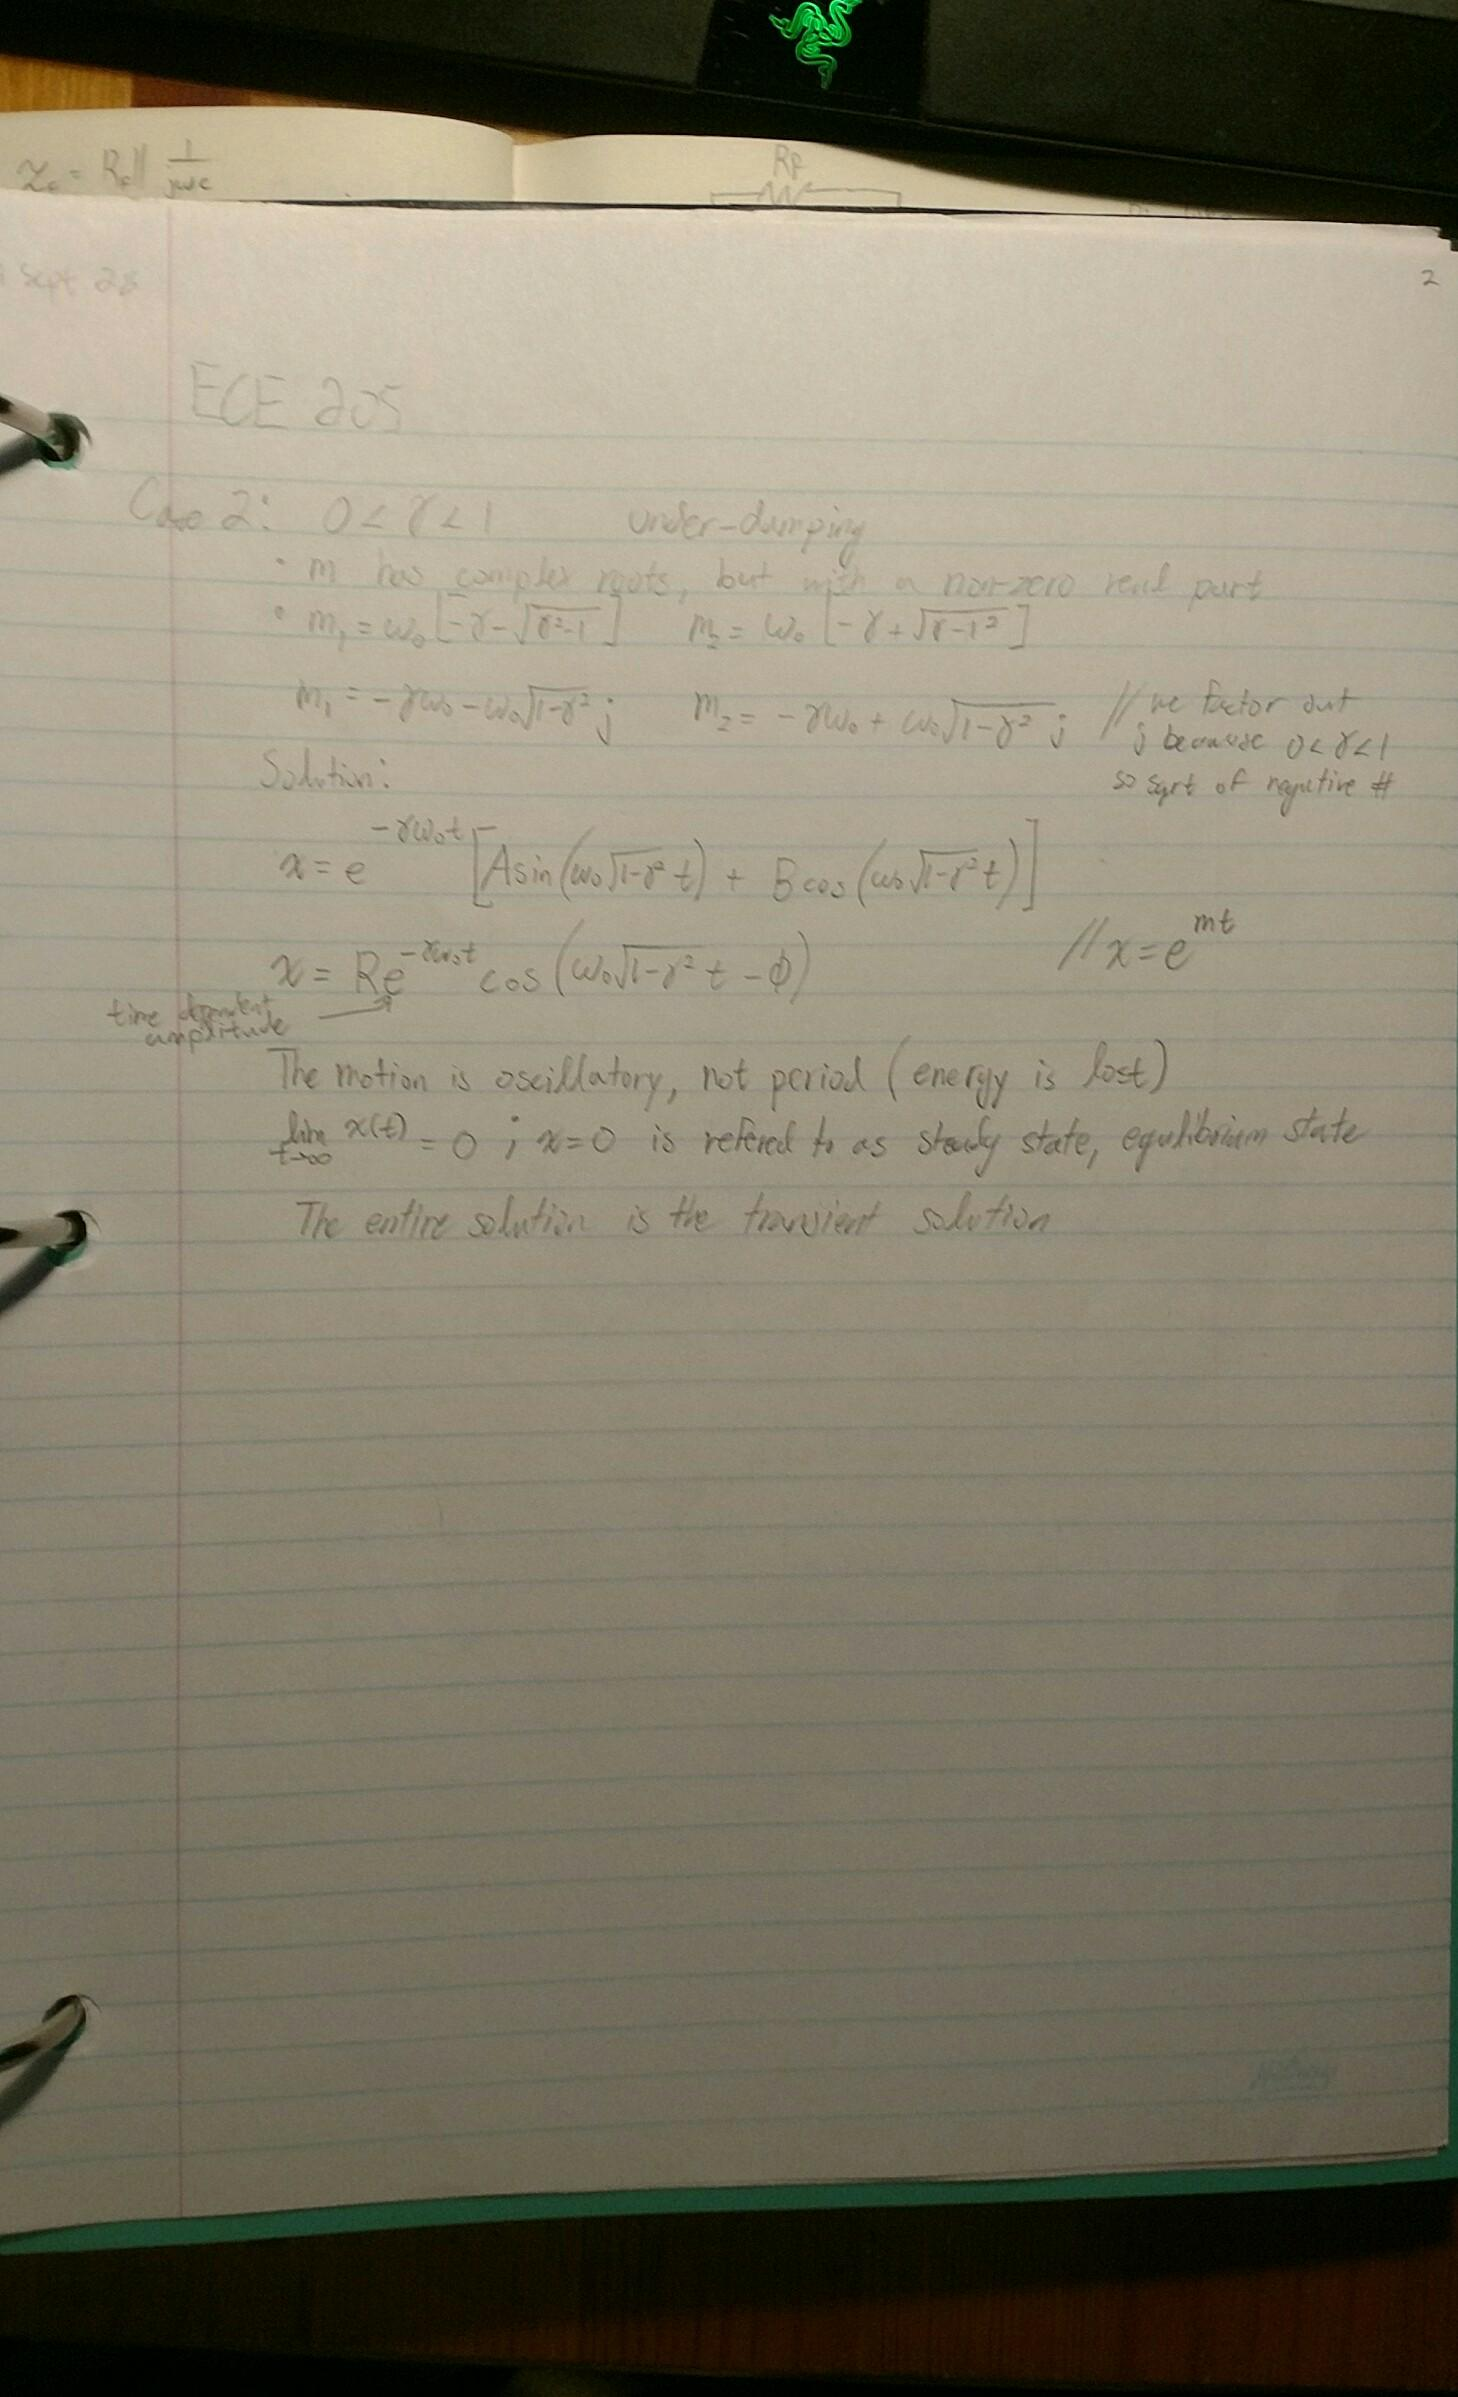
\includegraphics[width=\textwidth,height=\textheight,keepaspectratio]{friday/3.jpg}\\
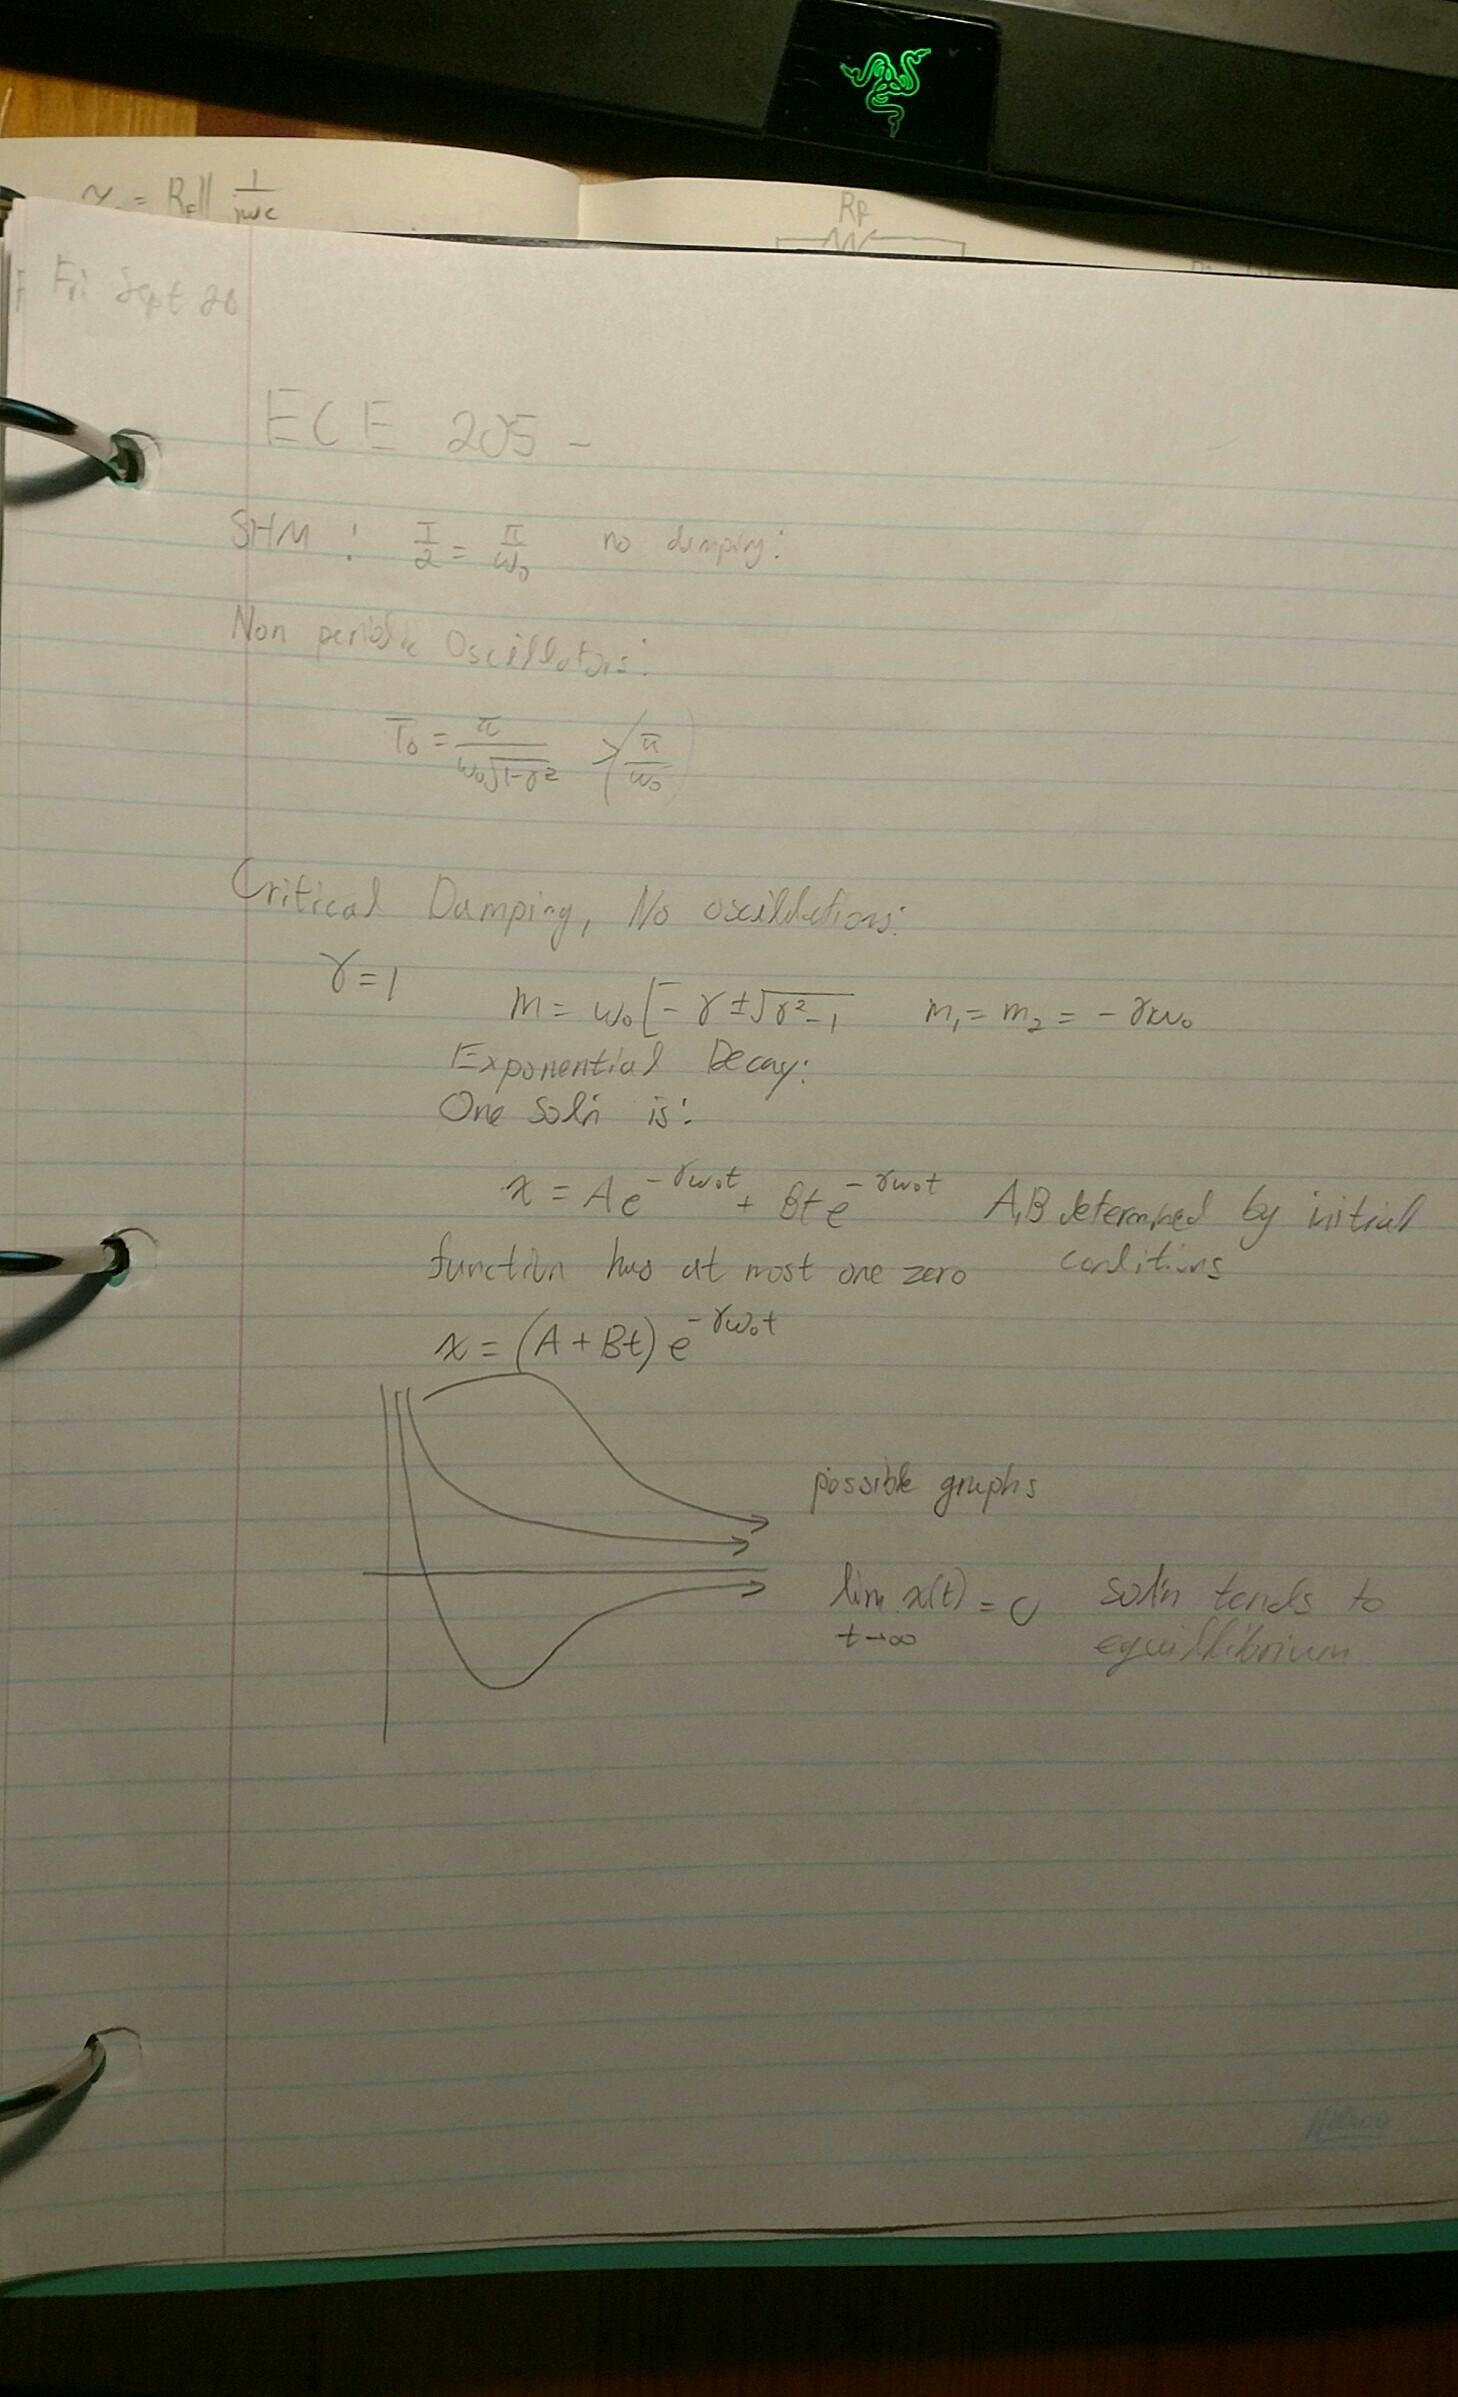
\includegraphics[width=\textwidth,height=\textheight,keepaspectratio]{friday/4.jpg}\\
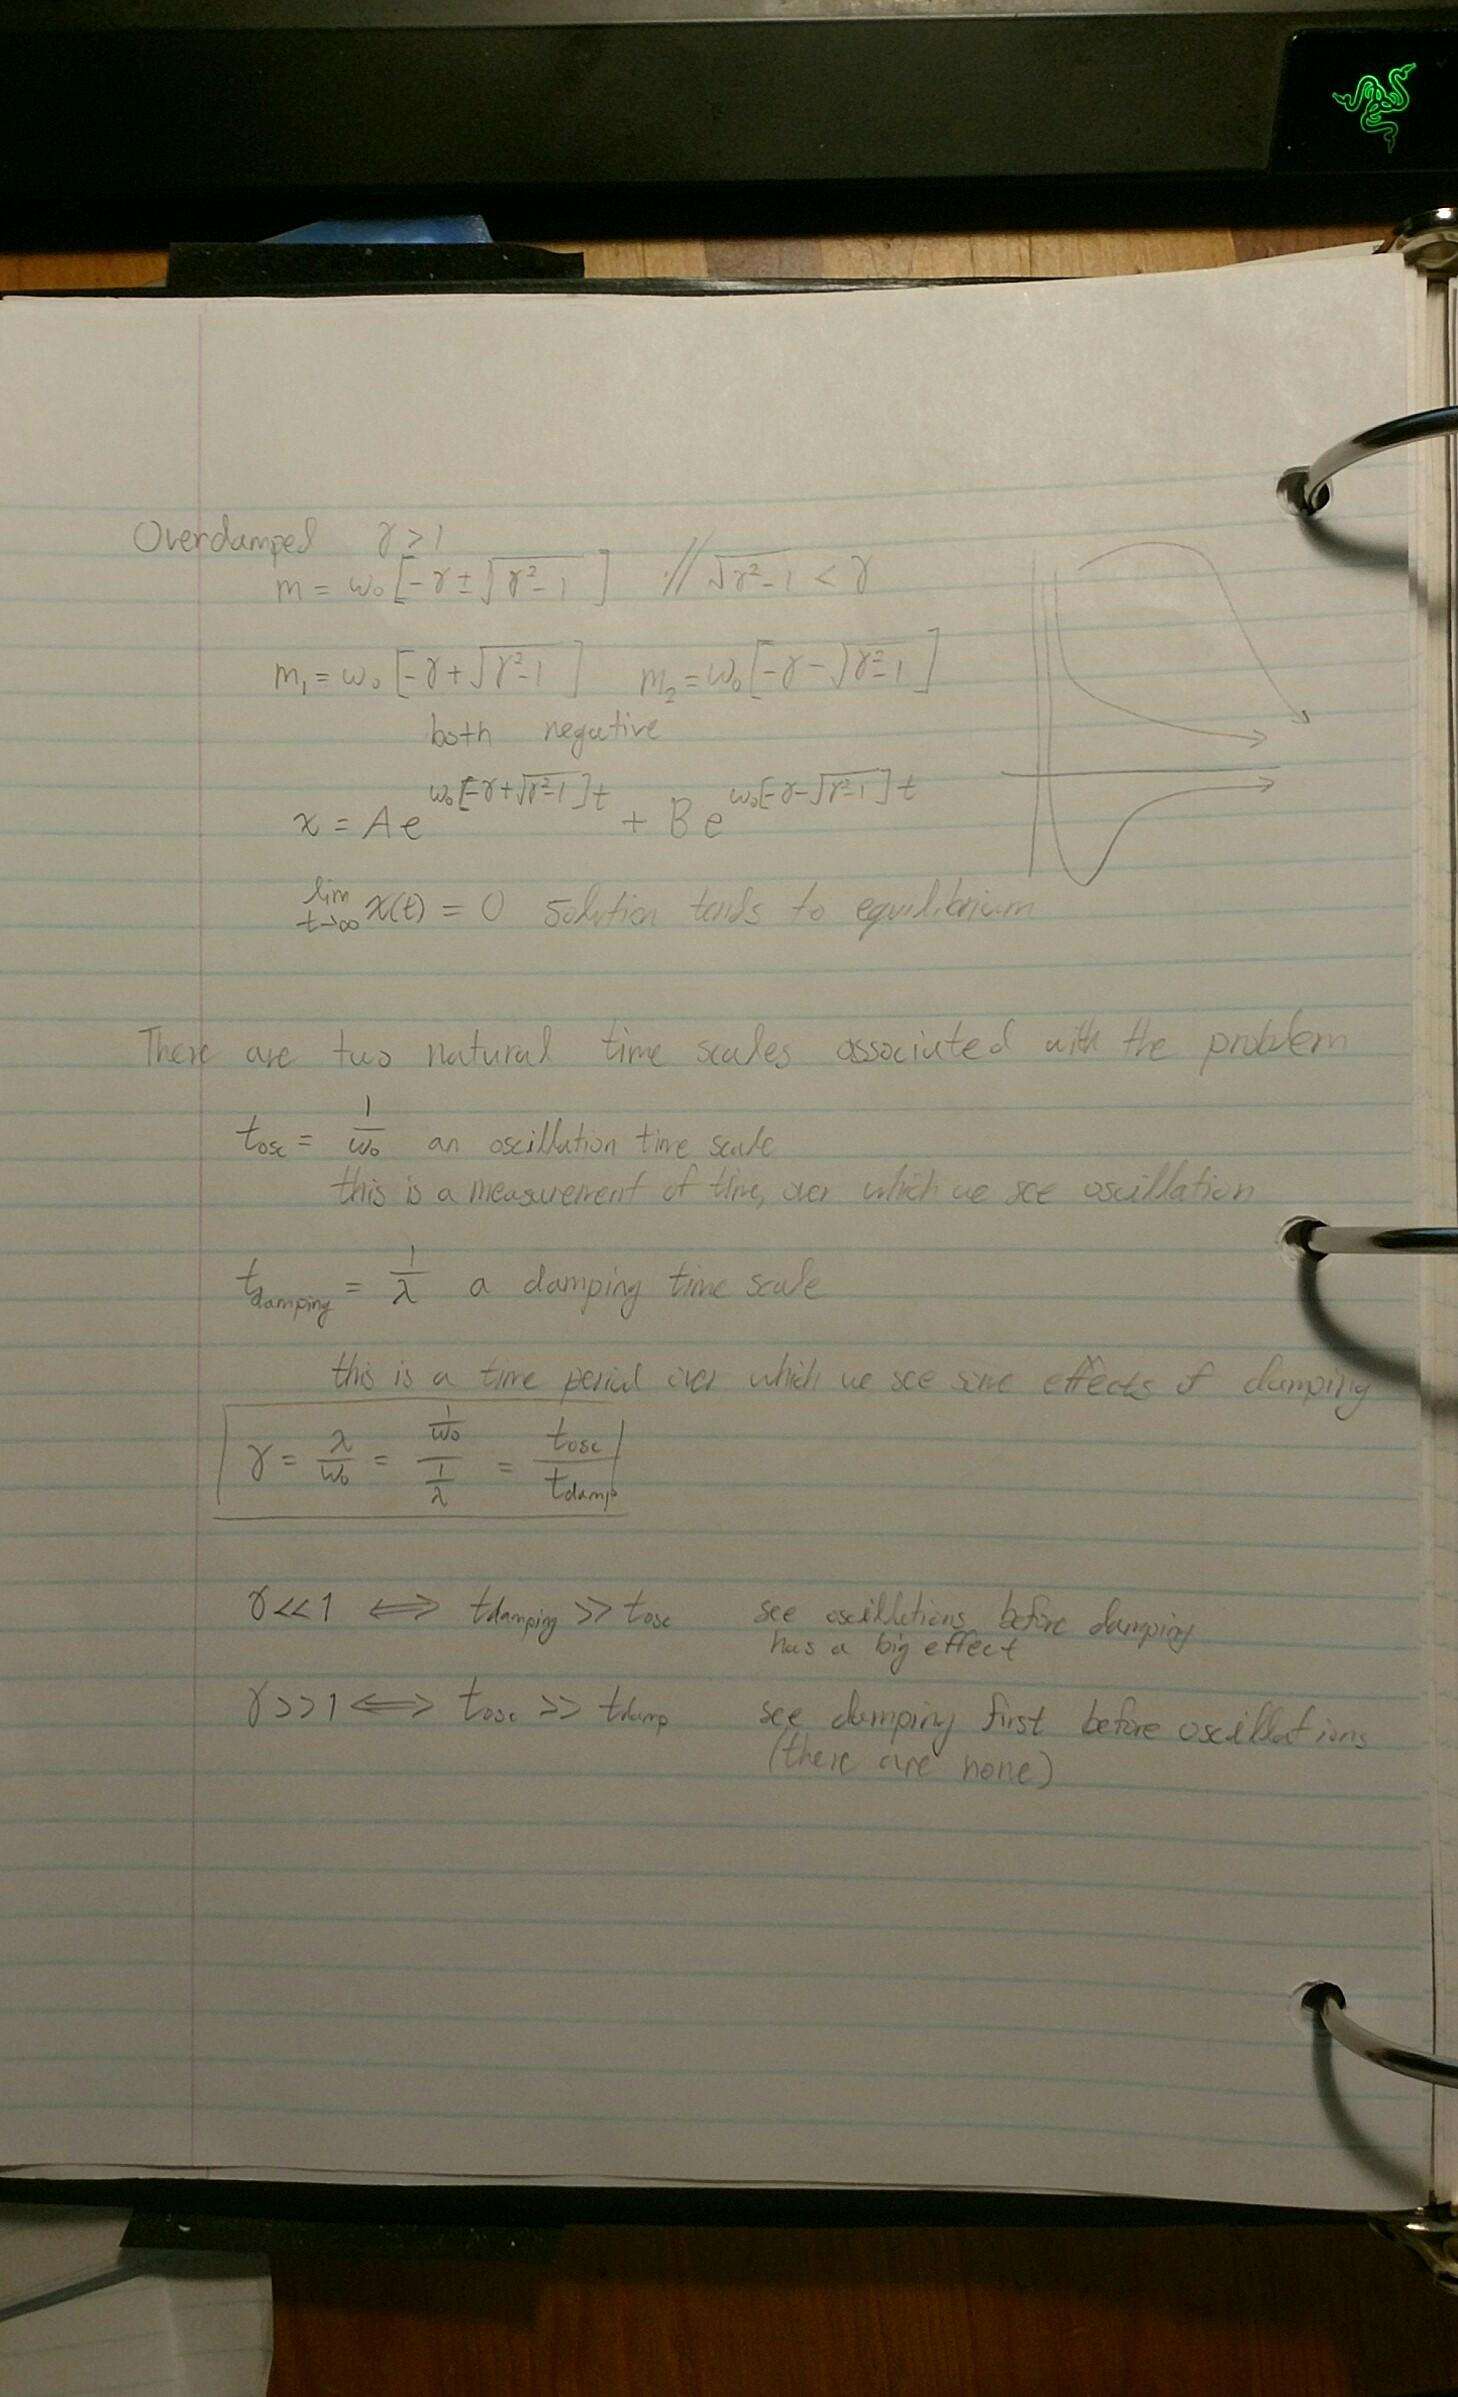
\includegraphics[width=\textwidth,height=\textheight,keepaspectratio]{friday/5.jpg}\\
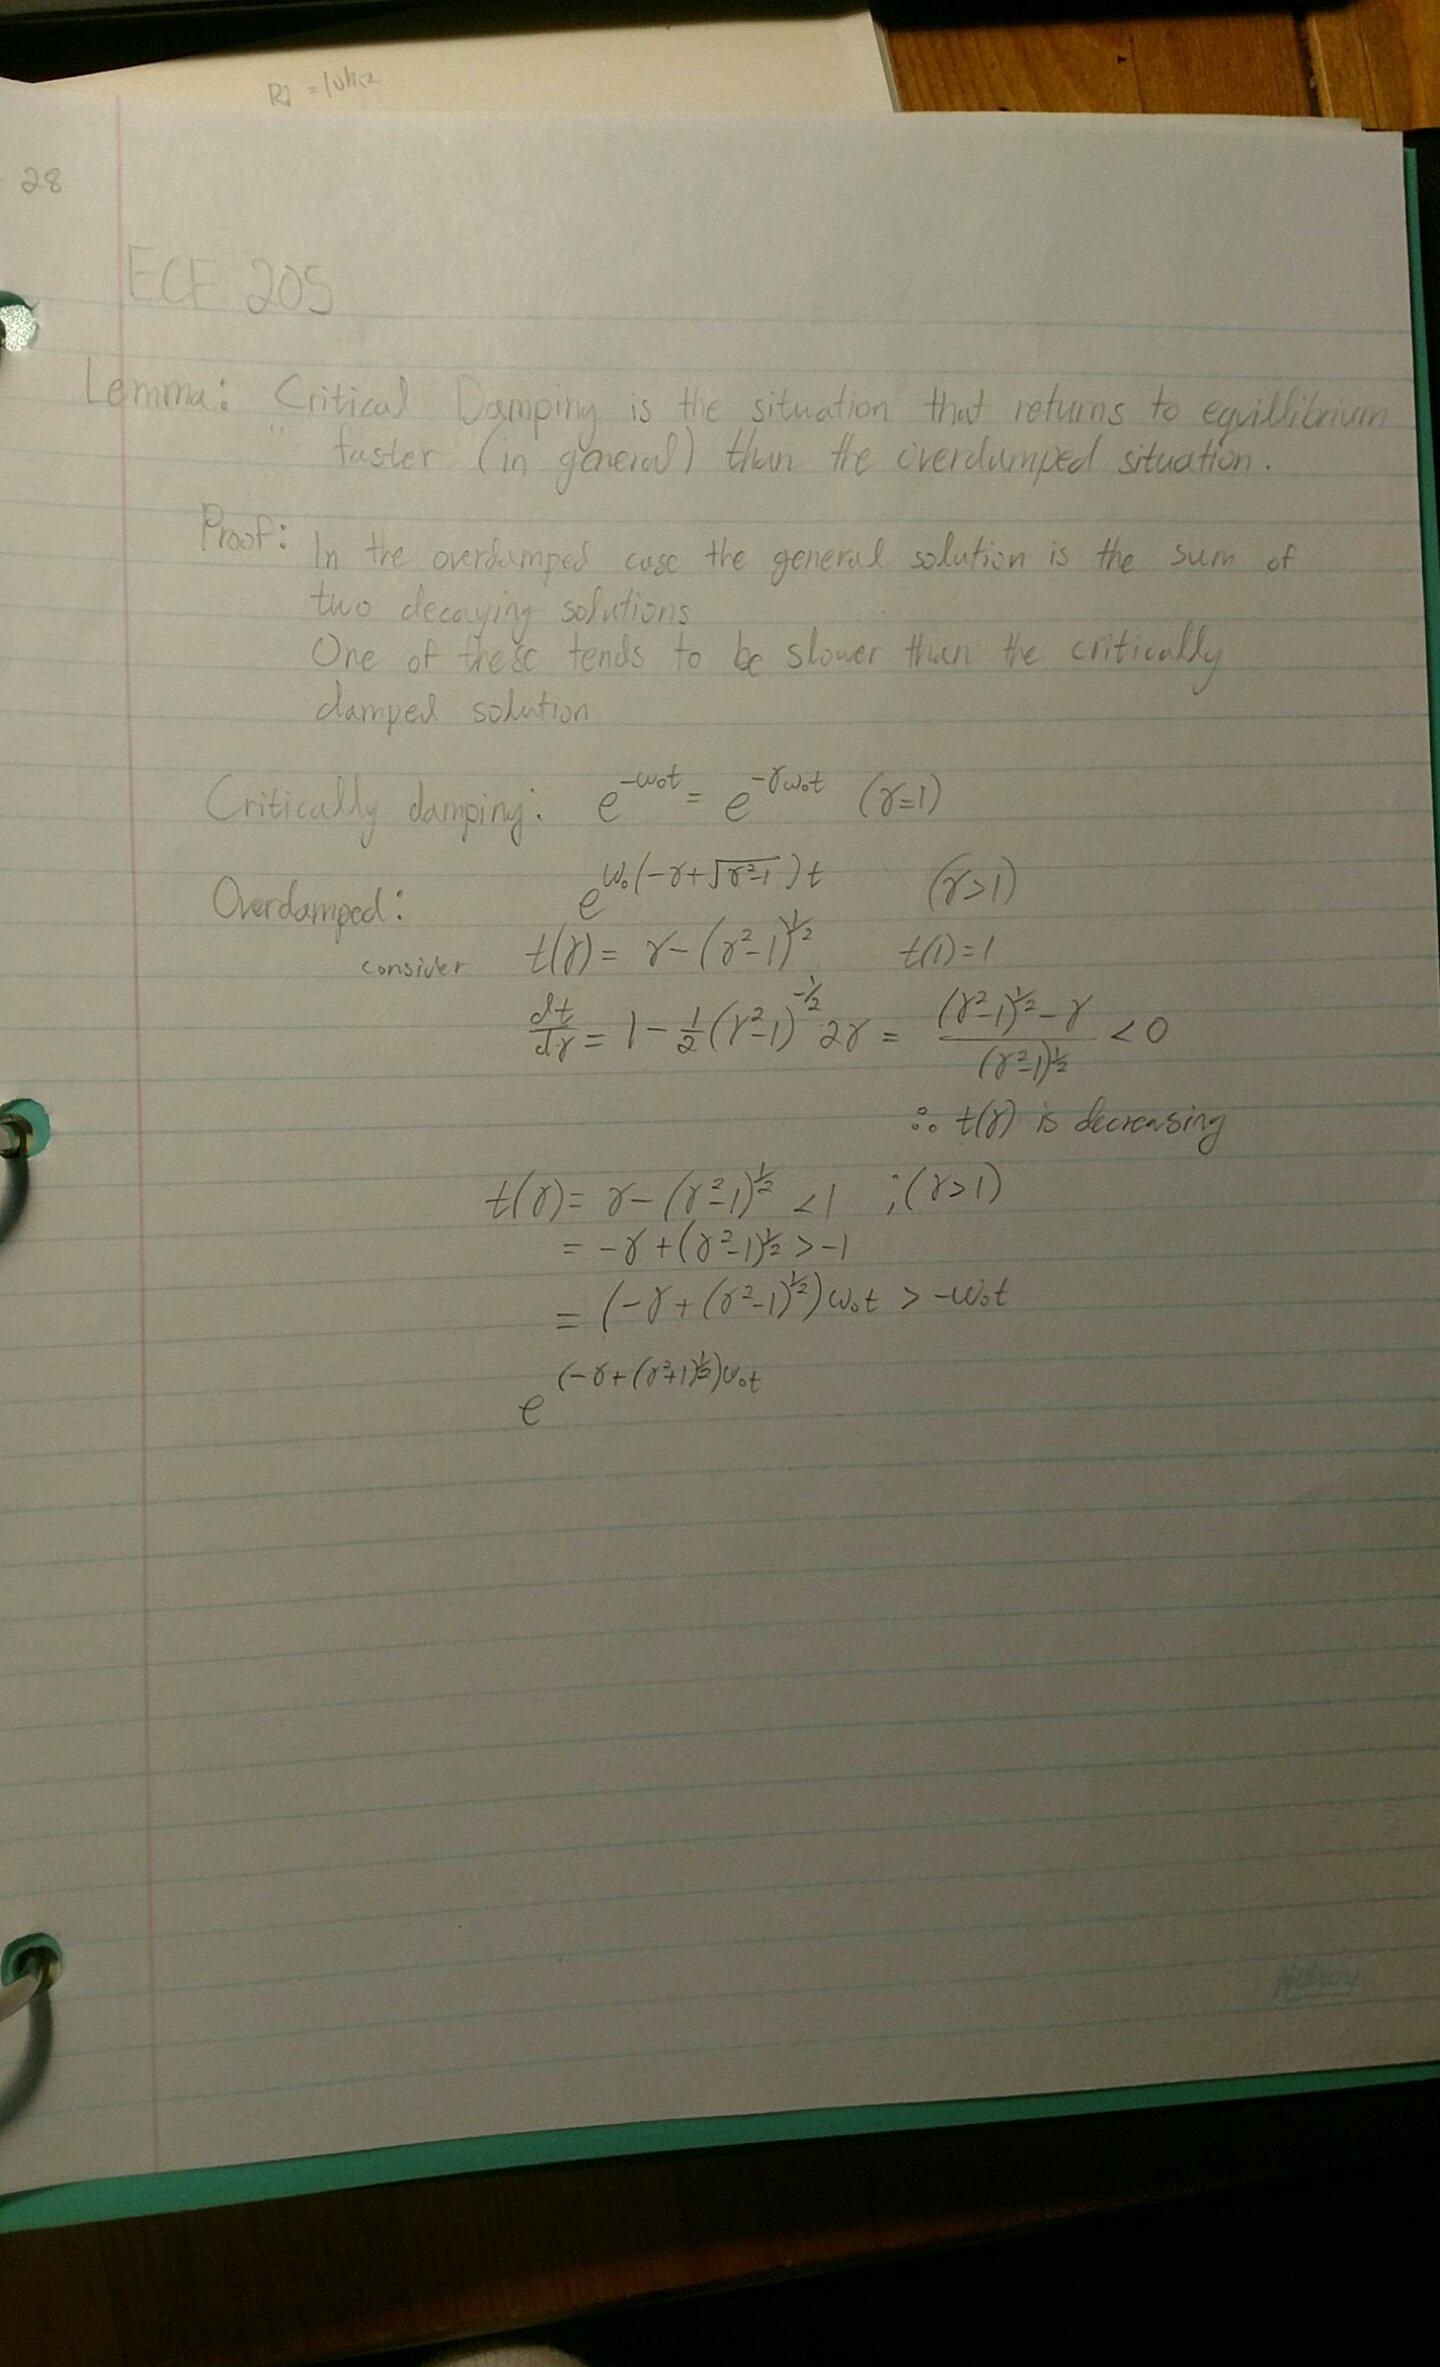
\includegraphics[width=\textwidth,height=\textheight,keepaspectratio]{friday/6.jpg}\\
\restoregeometry
\clearpage
\newpage

\textbf{Part 2: Driving term/ Forcing Term}
$$\ddot{x} + 2\lambda \dot{x} + \omega_0^2x = F(t)$$
$\omega_0$ is the natural frequency of the system.
We will consider $$F(t) = cos(\Omega t)$$
Comments:\begin{enumerate}[topsep=-10pt]
    \item In many circumstances we do have a periodic driving term
    \item Other functions can be decomposed into a linear combination of trig functions and we are looking at one piece of this decomposition.
    \textit{(see Fourier series)}
\subsubsection{Case A: No damping}
$$\ddot{x} + \omega_0^2x = F(t) = cos(\Omega t)$$
$x = x_H + x_P$ where $x_H$ solves $\ddot{x} + \omega_0^2x = 0$, $x_H = Rcos(\omega_0 t - \phi)$\\
\textbf{Case 1: $\Omega \neq \omega_0$}\\
$x_P = Asin(\Omega t) + Bcos(\Omega t)$\\
$\dot{x}  = \Omega[A cos\Omega t - Bsin\Omega t]$\\
$\ddot{x} = \Omega^2 [-x_p]$\\
Put into the DE to get
$$-\Omega^2x_p + \omega_0^2x_p = cos(\Omega t)$$
Thus
$$(\omega_0^2-\Omega^2)[Asin(\Omega t) + Bcos(\Omega t)] = 1\dot cos(\Omega t)$$\\
$A = 0, B = \frac{1}{\omega_0^2-\Omega^2}$\\
Thus the general solution is $x_p = \frac{1}{\omega_0^2-\Omega^2} cos(\Omega t)$\\
Which means $x = x_H + x_p = Rcos(\omega_0t + \phi) + \frac{1}{\omega_0^2-\Omega^2} cos(\Omega t)$\\
\textit{Special case, setting $\phi = 0$}\\
At which point $x = x_H + x_p = Rcos(\omega_0t) + \frac{1}{\omega_0^2-\Omega^2} cos(\Omega t)$\\
One special case arises when the two amplitudes are equal (or very close) $\implies R = \frac{1}{|\omega_0^2-\Omega^2|}$ or $R \approx \frac{1}{|\omega_0^2-\Omega^2|}$. The two contributions could cancel out for some time.\\
Adding the two $cos$ terms we get $x = R2[cos(\frac{(\omega_0 + \Omega)t}{2})cos(\frac{(\omega_0 - \Omega)t}{2})]$\\
This means that the second special case arises when the frequencies are almost the same, but not completely, which is why we get the following graph.\\
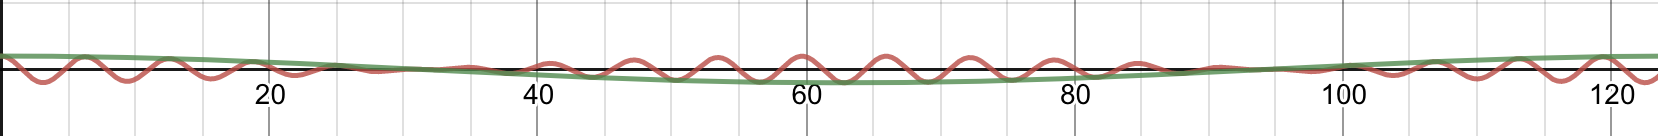
\includegraphics[width=\textwidth]{coscos.png}\\
This is called the phenomenon of \textbf{Beats}\\
\textbf{Case 2: $\Omega = \omega_0$}\\
$x_P = t(Asin(\Omega t) + Bcos(\Omega t))$
$$\dot{x_p} = Asin(\Omega t) + Bcos(\Omega t) + t\Omega(Acos(\Omega t) - Bsin(\Omega t))$$
$$\ddot{x_p} = 2\omega_o(Acos(\Omega t) - Bsin(\Omega t)) + t\omega_0^2(-Asin(\Omega t) - Bcos(\Omega t))$$
Put into the DE to get:
$$\ddot{x_p} + \omega_0^2x_p = 2\omega_o(Acos(\Omega t) - Bsin(\Omega t)) \equiv cos(\Omega t)$$
$\implies 2A\omega_0 = -1 \implies A = \frac{1}{2\omega_0}$\\
$\implies B = 0$\\
Thus $x_p = \frac{1}{2\omega_0}tsin(\omega_0 t)$\\
This has linear growth and it eventually breaks as visible from the graph on the next page
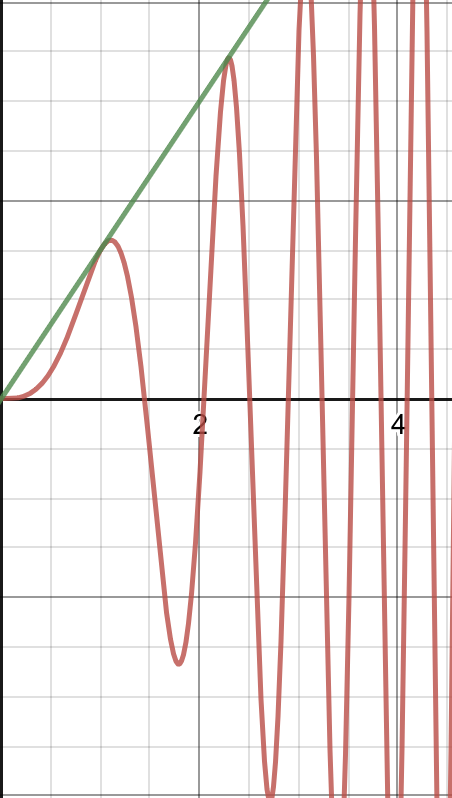
\includegraphics[width=0.5\textwidth]{resonance.png}
\end{enumerate}
\newpage


\textit{Lemma:} $L[t^nf(t)] = (-1)^n\frac{d^nF(s)}{ds^n}$, where $L[f(t)] = F(s)$

\newpage
\section{Fourier Series}
\subsection{Hyper applied linear algebra}
We're going to be looking in $C^\infty [-\pi, \pi]$, i.e. infinitely differentiable in $[-\pi, \pi]$ [Which is also infinite dimensional]

\textbf{Unique Representation Theorem:} Any vector in a given space can be represented in exactly one way using the given bases [There is only one way because the basis are all linearly independent]


To get from one base to another, there are 2 ways.
\begin{enumerate}[topsep=-10pt,itemsep=-5pt]
    \item Solve the equation
    \item Change of basis/co-ordinate matrix
    \item Orthogonal / Orthonormal basis
\end{enumerate}
\subsubsection{Ortho-normal Basis}

$B_1 = \{
\begin{pmatrix}
1\\
2\\
3\\
\end{pmatrix}, \begin{pmatrix}
4\\
5\\
6\\
\end{pmatrix}, \begin{pmatrix}
7\\
8\\
9\\
\end{pmatrix}\}$\\
$p$ and $q$ are orthogonal means $p . q = 0$\\
An orthogonal basis for $\R^n$ is one in which the vectors in the basis are mutually orthogonal. [The basis $B_1$ above is not orthogonal, while $B_2$ below is]\
$B_2 = \{
\begin{pmatrix}
1\\
2\\
3\\
\end{pmatrix}, \begin{pmatrix}
1\\
1\\
-1\\
\end{pmatrix}, \begin{pmatrix}
5\\
-4\\
1\\
\end{pmatrix}\}$\\


Let $z = [v_1, v_2, v_3$ is an orthogonal basis for $\R^3$. Let $v \epsilon \R^3$, $v = a_1v_1 + a_2v_2 + a_3v_3$\\
$v \cdot v1 = (a_1v_1 + a_2v_2 + a_3v_3)\cdot v$
$v\cdot v_1 = a_1v_1\cdot v_1$\\
$v \cdot v_2 = a_2v_2\cdot v_2$\\
$v \cdot v_3 = a_3v_3\cdot v_3$\\

We say that a basis $B = \{v_1, \dots v_p\}$ is an orthonormal basis to mean that:
\begin{enumerate}[topsep=-10pt,itemsep=-5pt]
    \item B is an orthogonal basis
    \item Each vector is a unit vector
\end{enumerate}

\subsubsection{Function Space}
Let $F(x)\; \epsilon\; C^\infty(-\pi,\; \pi)$\\
Taylor Series/Theorem: Basis = $\{1,x,x^2,x^3\dots x^n\}$\\
Fourier Basis: $\{1, cos(x), cos(2x), cos(3x) \dots cos(nx), sin(x), sin(2x), \dots sin(nx)\}$

$F(x) "=" \frac{1}{2}a_0 + a_1cos(1x) + a_2cos(2x) \dots + a_ncos(nx)$

Let $V$ be a vector space\\
A function $<, >: V \times V \rightarrow \C$ which satisfies:
$$<v,w> = \overline{<w,v>} \text{        Conjugate symmetry}$$
$$<a_1v_1 + a_2v_2,w> = a_1<v_1,w> + a_2<v_2,w> \text{        Linearity in 1st "slot"}$$
$$<v,v>\; \epsilon\; \R, <v,v>\; \geq 0\; \text{and}\; <v,v> = 0 \;\text{iff}\; v = 0  \text{        Non negativity}$$
We call $(V, <,>)$ is called an inner product sapce with $<,>$ is the inner product\\
The length of $v$ is $||v|| = \sqrt{<v,v>}$\\
eg: $\R^n$ vector space $v\cdot w = v_1w_1 + .....v_nw_n$ i.e the "dot product" is an inner product

Now considering $C^\infty [-\pi, \pi]$ and $f(x), g(x) \; \epsilon \; C^\infty (-\pi, \pi)$.\\ We define $<f(x), g(x)> = \int^\pi_{-\pi}f(x)g(x)dx$\\

Consider the basis $B = \{1, cosx, cos2x,....sin(x), sin(2x)....sin(mx)\}$ and these "vectors" are orthogonal.

$$<1,cosnx> = \int^\pi_{-\pi} 1cos(nx)dx = \frac{sin(nx)}{n}|^{\pi}_{-\pi} = 0$$

$$<1,sinmx> = \int^\pi_{-\pi} 1sin(mx)dx =
\frac{cos(mx)}{-m}|^{\pi}_{-\pi} = 0$$
If $m \neq n$,
$$<cos(mx),cos(nx)> = \int^\pi_{-\pi} cos(mx)cos(nx)dx = 0$$
$$<sin(mx),sin(nx)> = \int^\pi_{-\pi} sin(mx)sin(nx)dx = 0$$
$$<sin(mx),cos(nx)> = \int^\pi_{-\pi} sin(mx)sin(nx)dx = 0$$
Thus,  all of the pairs above are orthogonal

$$<1,1> = 2\pi$$
$$<sin(nx), sin(nx)> = \int^\pi_{-\pi} sin^2(nx) dx = \pi$$ $$<cos(nx), cos(nx)> = \int^\pi_{-\pi} cos^2(nx) dx = \pi$$

Thus we have an orthogonal basis, but not an orthonormal basis
\section{Fourier}
Let $h(x)\; \epsilon\; C^\infty (-\pi, \pi)$,
$$h(x) "=" \frac{1}{2}a_0 + \sum ^\infty_{k=1}a_kcos(kx) + \sum ^\infty_{m=1}b_msin(mx)$$

The constant term has half coefficient because of the 2 in $<1,1>$
$$a_0 = \frac{1}{\pi}<h(x), 1> = \frac{1}{\pi}\int^\pi_{-\pi} h(x)dx$$
$$a_k = \frac{1}{\pi}<h(x), cos(kx)> = \frac{1}{\pi}\int^\pi_{-\pi} h(x)cos(kx)dx$$
$$b_m = \frac{1}{\pi}<h(x), sin(mx)> = \frac{1}{\pi}\int^\pi_{-\pi} h(x)sim(mx)dx$$
The scalars $a_0, a_1, ....b_1, ...b_m$ are called the fourier coefficients of h(x)\\
Consider $h(x) = x$ on $(-\pi, \pi)$, and $h(x)$ is an odd function\\
$$a_0 = \frac{1}{\pi}\int^\pi_{-\pi}xdx = 0 \text{ since it is an odd function}$$\\
$$a_k = \frac{1}{\pi}\int^\pi_{-\pi}xcos(kx)dx = 0 \text{ since it is an odd function}$$\\
$$b_m = \frac{1}{\pi}\int^\pi_{-\pi}xsin(mx)dx = \frac{2}{\pi}\int^\pi_{0}xsin(mx)dx = \frac{2}{\pi}[\frac{xcos(mx)}{-m}|_0^\pi + \frac{1}{m}\int^\pi_0cos(mx)dx] = \frac{2}{\pi}\frac{\pi cos(m\pi)}{-m}$$
$$= 2(-1)^m/-m = \frac{2(-1)^{m+1}}{m}$$
Thus the fourier series for the function $x$ is
$$2[1sin(1x) -\frac{1}{2}sin(2x) + \frac{1}{3}sin(3x) -\frac{1}{4}sin(4x)+\dots + \frac{(-1)^{m+1}sin(mx)}{m}]$$
\subsection{Partial sums}
$$S_1 = 2sin(1x)$$
$$S_2 = 2[sinx - \frac{1}{2}sin(2x)]$$

\newpage
\textit{Notice:} The original function was defined on $(-\pi, \pi)$ but the Fourier series is defined on the whole of R and has period $2\pi$, so what does it converge to?\\
Let $F(x)$ be defined on $(-\pi, \pi)$. We define the $2\pi$ periodic extension of $F,\; F_p(x)$ as follows:
    $$F_p(x) = F(x)\;\;\;\; x \epsilon (-\pi, \pi)$$
    $$F_p(\pm\pi) = \frac{1}{2} [\lim_{x \to -\pi}F(x) + \lim_{x \to \pi}F(x)]$$
    $$F_p(x+2n\pi) = F_p(x)\; for\; all\; x\;\epsilon\; \R$$
    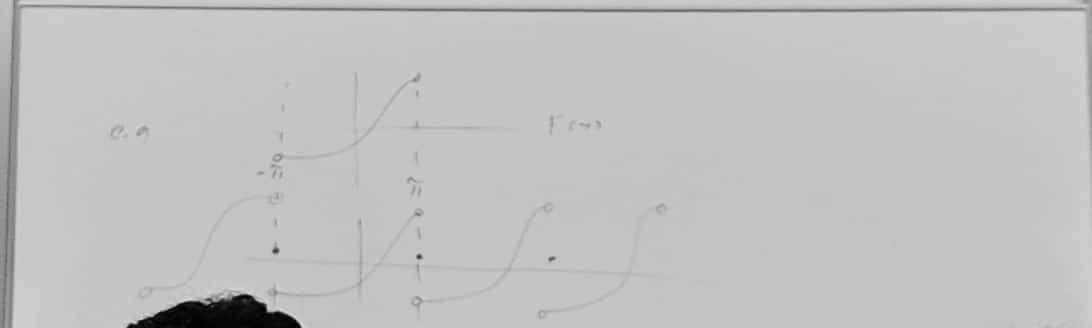
\includegraphics[width=\textwidth]{fourier1.jpg}\\

\textbf{Theorem:} Point-wise Convergence of Fourier Series\\
Suppose $G(x)$ has a period of $2\pi$ and is a piecewise in $\C'$ then:
\begin{enumerate}[topsep=-10pt]
    \item The Fourier series of $G(x)$ converges pointwise for all $x_0 \epsilon \R$:
    $$\frac{1}{2}a_0 + \sum ^\infty_{k=1}a_kcos(kx) + \sum ^\infty_{m=1}b_msin(mx) = N_{x_0}$$
    \item If $G(x)$ is continuous at $x_0$ then $N_{x_0} = G(x_0)$
    \item If $G(x)$ is not continuous at $x_0$ then $N_{x_0} = \frac{1}{2} [\lim_{x \to x_0^-}F(x) + \lim_{x \to x_0^+}F(x)]$
\end{enumerate}
In particular the Fourier Series of a function $F(x)$   $[C']$ defined on $(-\pi, \pi)$ will converge to $F_p(x_0)$ at points where $F_p(x)$ is continuous and to the midpoint at points where $F_p(x)$ is not continuous\\
\textit{Note:} We have an infinite sum of continuous functions \textbf{\underline{BUT}} the sum is not continuous\\
Suppose $F(x)$ is defined on $(-L, L)$ instead of $(-\pi, \pi)$\\
Our Basis become: $$\{1, cos\frac{n\pi x}{L}, sin\frac{m\pi x}{L}\}$$\\
$F(x)$ becomes: $$F(x) = \frac{1}{2}a_0 + \sum ^\infty_{k=1}a_kcos(\frac{k \pi x}{L}) + \sum ^\infty_{m=1}b_msin(\frac{m \pi x}{L})$$

$$a_k = \frac{1}{L}\int^L_{-L}F(x)cos(\frac{k \pi x}{L})dx$$\\
$$b_k = \frac{1}{L}\int^L_{-L}F(x)sin(\frac{k \pi x}{L})dx$$\\

In a periodic is often have $F(x)$ on $[0,L)$ and we want a fourier series for this\\

We will extend $F(x)$ there are 5 ways:\\
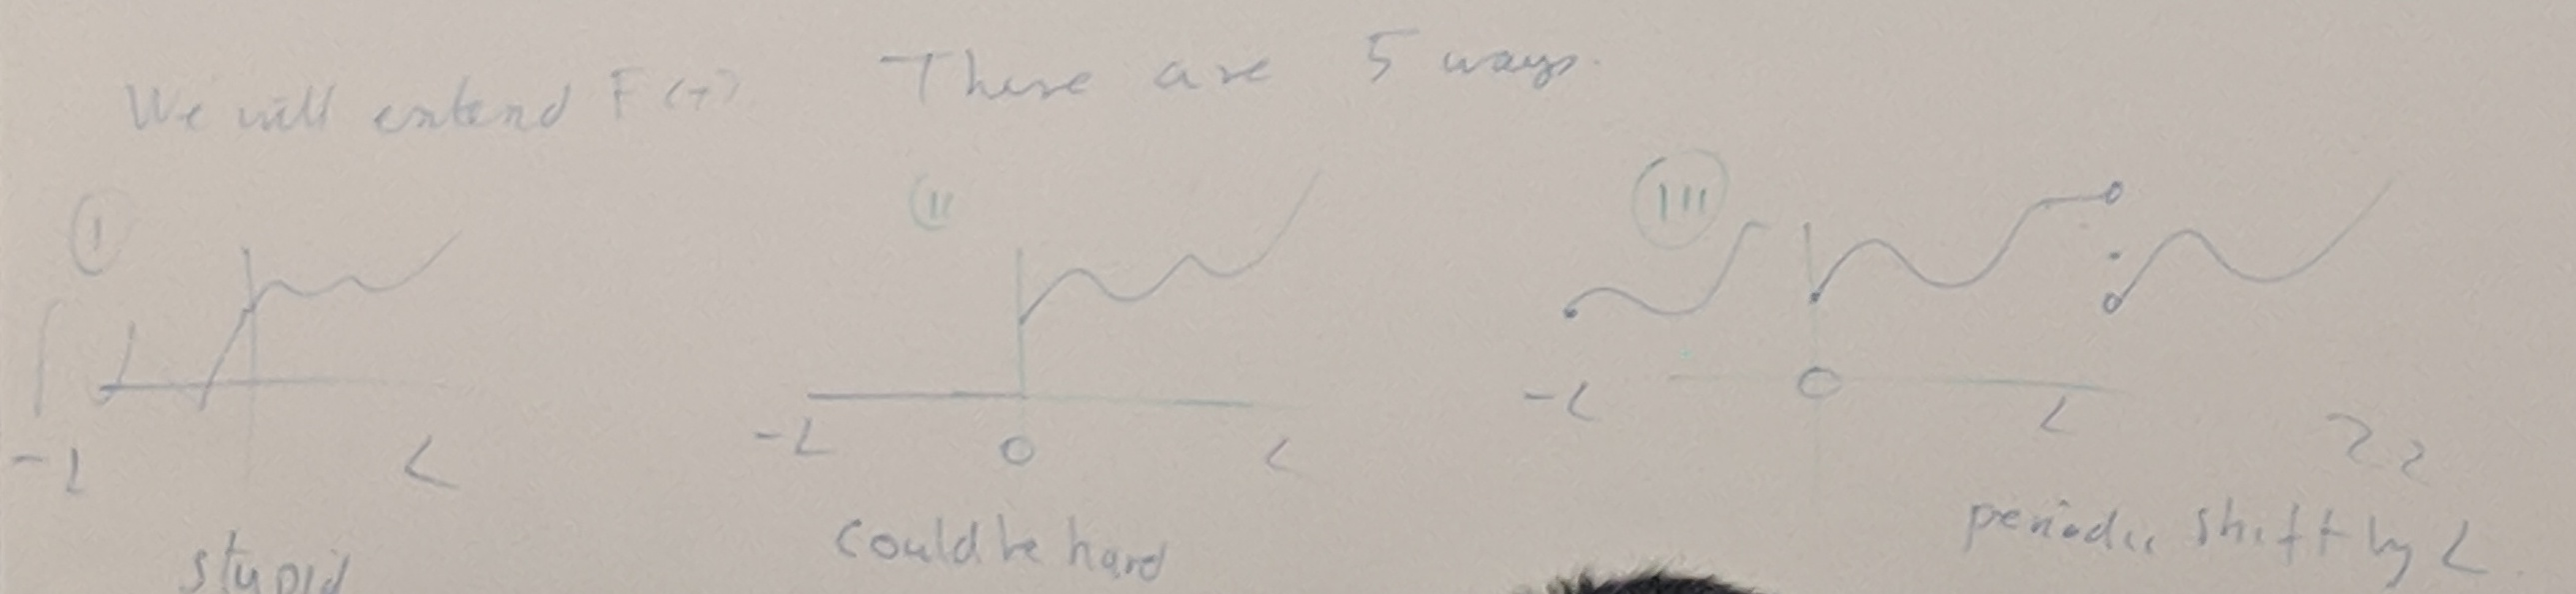
\includegraphics[width=\textwidth]{MVIMG_20181109_102732.jpg}\\

$$x = 2[sinx -\frac{sin2x}{2} + \frac{sin3x}{3} + \dots] \text{ on } [-\pi, \pi]$$
$$\implies \frac{\pi}{2} = 2[1 - \frac{1}{3} + \frac{1}{5} \dots]\implies \frac{\pi}{4} = \sum^\infty_{n=0} \frac{(-1)^n}{2n + 1}$$



If $F(x)$ is defined on $(0,\pi)$\\
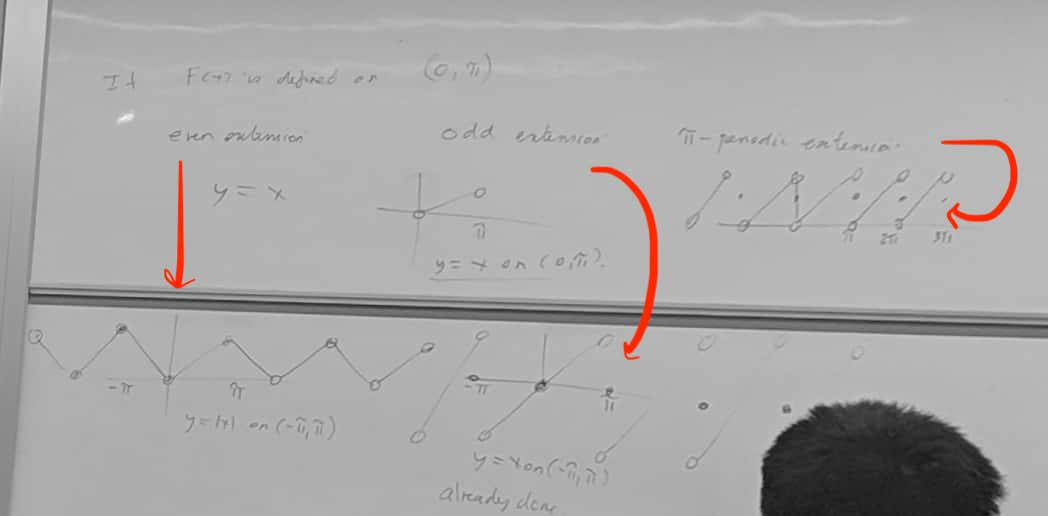
\includegraphics[width=\textwidth]{extensions.jpg}\\

Even Extension: $y = |x| \text{ on } (-\pi,\pi)$, $b_n = 0 \forall n$\\
$a_0 = \frac{1}{\pi}\int^\pi_{-\pi}|x|dx = \pi$\\
$a_n = \frac{1}{\pi}\int^\pi_{-pi} |x|cos(n\pi x)dx$, $n = 1,2,3$\\
$a_n = \frac{2}{\pi}\frac{cos(n\pi x)}{n^2}|^\pi_0 = \frac{2}{\pi n^2}[(-1)^n -1]$, $n = 1,2,3$\\
$a_n = 0$, when n is even, and is $-\frac{4}{\pi n^2}$\\
$F(x) = \frac{\pi}{2} - \frac{4}{\pi}[\frac{cosx}{1^2} + \frac{cos3x}{3^2} + \dots]$\\
$$F(x) = \frac{\pi}{2} - \frac{4}{\pi}\sum_{n=0}^\infty\frac{cos(2n+1) x}{(2n+1)^2}$$\\
$\pi$ Periodic Extension: There are two ways for this\\
\[F(x) =  \begin{cases}
      x & (0,\pi) \\
      x+\pi & (-\pi, 0) \\
      2.5 & x = 0
   \end{cases}
\]
\textbf{OR WE CAN DO}
\[F(x) =  \begin{cases}
      x & (0,\pi/2) \\
      x+\pi & (-\pi/2, 0) \\
      0 & x = 0
   \end{cases}
\]\\

$$F(x) = \frac{1}{2}a_0 + 2 a_n cos\frac{n\pi x}{\pi/2} + 2 b_n sin\frac{n\pi x}{\pi/2}$$
$$F(x) = \frac{1}{2}a_0 + 2 a_n cos(2n x) + 2 b_n sin(2n x)$$

$$a_0 = \frac{2}{\pi}\int^{\frac{\pi}{2}}_{\frac{-\pi}{2}}F(x)dx = \frac{2}{\pi}[\int^0_{-\pi/2}(x+\pi)dx + \int^{\pi/2}_0(x)dx] = \pi$$
$$a_n =  \frac{2}{\pi}\int^{\frac{\pi}{2}}_{\frac{-\pi}{2}}F(x)cos(2nx)dx = \frac{2}{\pi}[\int^{0}_{\frac{-\pi}{2}}(x+\pi)cos(2nx)dx + \int^{\frac{\pi}{2}}_{0}xcos(2nx)dx]$$
$$\implies \frac{2}{\pi}[\int^{\frac{\pi}{2}}_{\frac{-\pi}{2}} xcos(2nx)dx + \int^{0}_{\frac{-\pi}{2}}\pi cos(2nx)dx] = 0$$
$$b_n =  \frac{2}{\pi}\int^{\frac{\pi}{2}}_{\frac{-\pi}{2}}F(x)sin(2nx)dx = \frac{2}{\pi}[\int^{0}_{\frac{-\pi}{2}}(x+\pi)sin(2nx)dx + \int^{\frac{\pi}{2}}_{0}xsin(2nx)dx]$$
$$\implies \frac{2}{\pi}[\int^{\frac{\pi}{2}}_{\frac{-\pi}{2}} xsin(2nx)dx + \int^{0}_{\frac{-\pi}{2}}\pi sin(2nx)dx] = \frac{2}{\pi}[2(\frac{xcos(2nx)}{-2n})|_0^{\frac{\pi}{2}} + \frac{1}{2n}\int^{\frac{\pi}{2}}_0 cos(2nx)dx + \pi \frac{cos(2nx)}{-2n}|^0_{\frac{-\pi}{2}}] = \frac{-1}{n}$$

$$\implies F(x) = \frac{\pi}{2} - \sum^\infty_1 \frac{sin(2nx)}{n}$$

\newpage
Consider a function with period $\tau$ defined on $[-\frac{\pi}{2}, \frac{\pi}{2}]$, $2\pi \rightarrow \tau$ i.e. $2L = \tau$
$$F(t) = \frac{1}{2}a_0 + \sum^\infty_1 a_nsin(\frac{2n\pi t}{\tau}) + \sum^\infty_1 b_ncos(\frac{2n\pi t}{\tau})$$
$$a_n = \frac{2}{\tau}\int^{\frac{\tau}{2}}_{\frac{-\tau}{2}}F(t) cos(\frac{2n\pi t}{\tau})dt$$
$$\omega_0 = \frac{2\pi}{\tau} \text{ [It is called the fundamental angular frequency]}$$
$$n\omega_0 \text{[These are called the harmonics]}$$
$$a_n = \frac{\omega_0}{\pi} \int^{\frac{\tau}{2}}_{\frac{-\tau}{2}}F(t) cos(n\omega_0t)dt$$
$$b_n = \frac{\omega_0}{\pi} \int^{\frac{\tau}{2}}_{\frac{-\tau}{2}}F(t) sin(n\omega_0t)dt$$
\\
We will complexify all this:\\
Consider the space of complex valued differentiable function defined on $[-\frac{\tau}{2}, \frac{\tau}{2}]$ (this is a vector space).\\
In this space we define the inner product as:
$$<F,G> = \int^{\frac{\tau}{2}}_{\frac{-\tau}{2}} F(t)\overline{G(t)}dt$$
In this space a basis is $\{1, e^{\iu n\omega_0 t}\}_{n\; \epsilon\; \Z}$ which is orthogonal i.e.
$$<e^{\iu n\omega_0 t}, e^{\iu m\omega_0 t}> = \int^{\frac{\tau}{2}}_{\frac{-\tau}{2}} e^{\iu n\omega_0 t} e^{-\iu m\omega_0 t}dt = \int^{\frac{\tau}{2}}_{\frac{-\tau}{2}} e^{\iu (n-m)\omega_0 t}dt = \frac{e^{\iu(n-m)\omega_0t}}{\iu (n-m)\omega_0}|^\frac{\tau}{2}_{-\frac{\tau}{2}} = 0 \text{ given }m \neq n$$
$$<1,1> = \int^{\frac{\tau}{2}}_{\frac{-\tau}{2}} 1dt = \tau$$
$$||e^{\iu n\omega_0 t}|| =  <e^{\iu n\omega_0 t}, e^{-\iu n\omega_0 t}> = \int^{\frac{\tau}{2}}_{\frac{-\tau}{2}} e^0dt = \tau$$\\
Let function $F(t)$ be a function in the vector space. We define the complex Fourier Series of $F(t)$ as follows
$$\sum^\infty_{n=-\infty}C_ne^{
\iu n\omega_0t} \text{   = F(t) for most of the time}$$

where $C_n = \frac{1}{\tau} \int^{\frac{\tau}{2}}_{\frac{-\tau}{2}} F(t)e^{-\iu n \omega_0t} dt$, $C_n = \frac{1}{\tau} <F(t), e^{\iu n \omega_0 t}>$\\
If $F(t)$ is real valued: $\overline{C_n} = \frac{1}{\tau} \int^{\frac{\tau}{2}}_{\frac{-\tau}{2}} F(t)e^{-\iu (-n) \omega_0t} dt = -C_n$

eg: $\omega_0 = 1$, $t \text{ on } (-\pi, \pi)$, $\tau = 2\pi$\\
$C_0 = \frac{1}{2\pi} \int^\pi_{-\pi}tdt = \frac{1}{2\pi}\frac{1}{2}(\pi^2 - (-\pi)^2) = 0$\\
$n \neq 0$\\
$C_n = \frac{1}{2\pi} \int^\pi_{-\pi}t e^{-\iu n t}dt = \frac{1}{2n\pi \iu}[\pi e^{-\iu n \pi } - -\pi e^{-\iu n (-\pi) }] + \frac{1}{2n\pi \iu}\frac{1}{-\iu n}[e^{-\iu n \pi } - e^{-\iu n (-\pi) }] = \frac{(-1)^n}{- \iu j} + \frac{1}{2n^2\pi}[0]\\ \implies C_n =  \frac{(-1)^n}{- \iu j} = \frac{(-1)^n\iu}{n}$

We can also show that $C_{-n} = C_n$\\
Complex Fourier Series: $$\sum_{n = 1}^\infty (\frac{-1^n}{n}\iu)e^{n\iu t} + \sum_{n = -1}^{-\infty} (\frac{-1^n}{n}\iu)e^{n\iu t}$$
If the second sum let $m = -n$
$$\sum_{n = 1}^\infty (\frac{(-1)^n}{n}\iu)e^{n\iu t} - \sum_{m = 1}^{\infty} (\frac{(-1)^m}{m}\iu)e^{m\iu t}$$
$$\sum_{n = 1}^\infty (\frac{(-1)^n}{n}\iu)\frac{e^{n\iu t} - e^{-n \iu t}}{2\iu}2\iu$$
$$2\sum\frac{(-1)^{n+1}}{n}sin(nt)$$

\newpage
\textbf{Complex Fourier Series}\\
$f(t)$ is $\tau$ periodic and $f(t)$ is defined on $[-\frac{\tau}{2}, \frac{\tau}{2}]$ with $\omega_0 = \frac{2\pi}{\tau}$
Basis: $\{1, e^{jn\omega_0}t\}$
$$\sum_{n=-\infty}^\infty C_n e^{jn\omega_0 t}$$
$$C_n = \frac{1}{\tau}\int^\frac{\tau}{2}_{-\frac{\tau}{2}}f(t)e^{-jn\omega_0 t}dt$$
If the function $f(t)$ is real $C_{-n} = \overline{C_n}$\\
\textit{Eg:} $\omega_0 = 1$, $t \text{ on } (-\pi, \pi)$, $\tau = 2\pi \implies C_n = \frac{(-1)^nj}{n}$\\
\textbf{Relationship between real and complex fourier series}
\begin{enumerate}[topsep=-10pt]
    \item $f(t) = \frac{1}{2}a_0 + \sum a_n cos(n\omega_0 t) + \sum b_n sin(n\omega_0 t)$
    \item $f(t) = \sum_{n=-\infty}^\infty C_n e^{nj\omega_0 t}$
\end{enumerate}
Using these we can get the result: $C_n = \frac{1}{2}(a_n - jb_n)$ and the other way: $a_n = (C_n + \overline{C_n}) = (C_n + {C_{-n}})$ and $b_n = \frac{1}{j}(\overline{C_n} - C_n) = j(C_n - \overline{C_n})$\\
\hfill\break

\textit{In a vector space with a basis $B$, if $\underline{v} \epsilon V$ and we know the components of $\underline{v}$ in B then we know everything about $\underline{v}$}\\
Suppose we have the complex Fourier coefficients of $f(t)$ then we know everything about $f(t)$\\
$C_n\; \epsilon\; \C$ and $C_n = |C_n|e^{i\phi}$ where $|C_n|$ is the magnitude and $\phi$ is the phase.\\
The set $\{C_n\}$ is sometimes called the Fourier Spectrum of  $f(t)$\\
The set $\{|C_n|\}$ is called the amplitude spectrum
$\overline{C_n} = |C_n|e^{-i\phi} = C_{-n}$\\
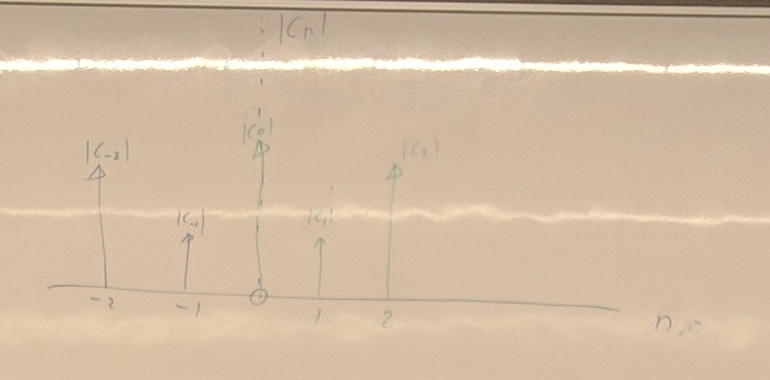
\includegraphics[width=0.8\textwidth]{MVIMG_20181113_085445.jpg}\\
Also, the strength of the signal can be defined by $\sum_{n=-\infty}^\infty |C_n|^2 $\\
This spectrum illustrates the relative importance of the contribution to $f(t)$ i.e. if $|C_p|$ then both $e^{j\omega_0 pt}$ and $e^{-j\omega_0 pt}$ play an important role in construction of $f(t)$ [equivalently $sin(p\omega_0 t) or cos(p\omega_0 t)$ have large co-efficients]\\
\hfill\break
\textbf{Parseval's Theorem:} Let $f(t)$ be a $\tau$ periodic function with $f(t) = \sum_{n=-\infty}^\infty C_n e^{nj\omega_0 t} $\\
Then, $<f(t), f(t)> = \int^{\frac{\tau}{2}}_{\frac{-\tau}{2}} f(t)\overline{f(t)}dt = \tau \sum_{n=-\infty}^\infty |C_n|^2$

\begin{quote}
If you take the inner product of the function then you get the sum of the squares of the components, with $\tau$ being added for not having the magnitudes not equal to 1
\end{quote}
Eg: $t$ on $(-\pi, \pi)$ with $C_n = \frac{(-1)^n}j{n}$ and $C_0 = 0$\\
$$<t, t> = \int^\pi_{-\pi}t^2dt = 2\pi \sum_{-\infty}^\infty = 2\pi [\sum_{-\infty}^{-1}\frac{1}{n^2} + \sum_1^\infty\frac{1}{n^2}]$$
$$\implies \int_{-\infty}^\infty t^2 dt = \frac{t^3}{3}|^\pi_{-\pi} = \frac{2\pi^3}{3} = 2\pi \times 2 \sum_{n =1}^\infty \frac{1}{n^2} \implies \sum_{n =1}^\infty \frac{1}{n^2} = \frac{\pi^2}{6}$$

\clearpage
\subsection{Fourier Transformation}
\textbf{Fourier Transform $f(t)$}\\
need a square integrable function $\int^{\infty}_{-\infty}|f(t)|^2dt$ is finite\\
$$F(\omega) = \int^{\infty}_{-\infty} f(t)e^{-j\omega t}dt$$
\textbf{Fourier Integral $F(\omega)$}\\
$$f(t) = \frac{1}{2\pi}\int^{\infty}_{-\infty} F(\omega)e^{j\omega t}d\omega$$

\textit{Example:}
Window function i.e. rectangular pulse\\
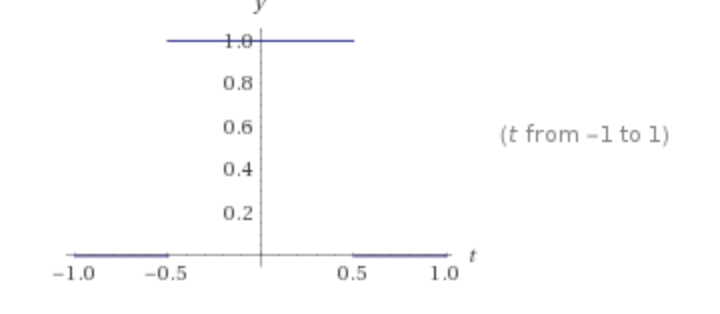
\includegraphics[width=0.8\textwidth]{windowfunction.png}\\
$$f(t) = H(t+\frac{1}{2}) - H(t-\frac{1}{2})$$
$$F(\omega) = \int^{\infty}_{-\infty} f(t) e^{-j\omega t}dt = \int_{-\frac{1}{2}}^{\frac{1}{2}}1e^{-j\omega t}dt = \frac{e^{-j\omega t}}{-j \omega}|^\frac{1}{2}_{-\frac{1}{2}} = \frac{2}{\omega}[\frac{e^{\frac{j\omega}{2}} - e^{-\frac{j\omega}{2}}}{2j}] = \frac{sin \frac{\omega}{2}}{\frac{\omega }{2}} = sinc(\frac{\omega}{2})$$
$$[\frac{sinx}{x} = sinc(x), \text{Sinch of x}]$$\\
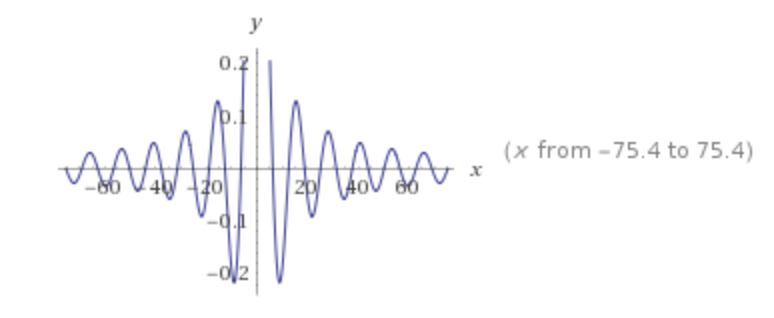
\includegraphics[width=0.8\textwidth]{sincx.png}\\

\subsubsection{Ad Hoc Derivation of the Fourier Integral}
Suppose we have a function which is defined on $[-\frac{\tau}{2}, \frac{\tau}{2}]$
\\
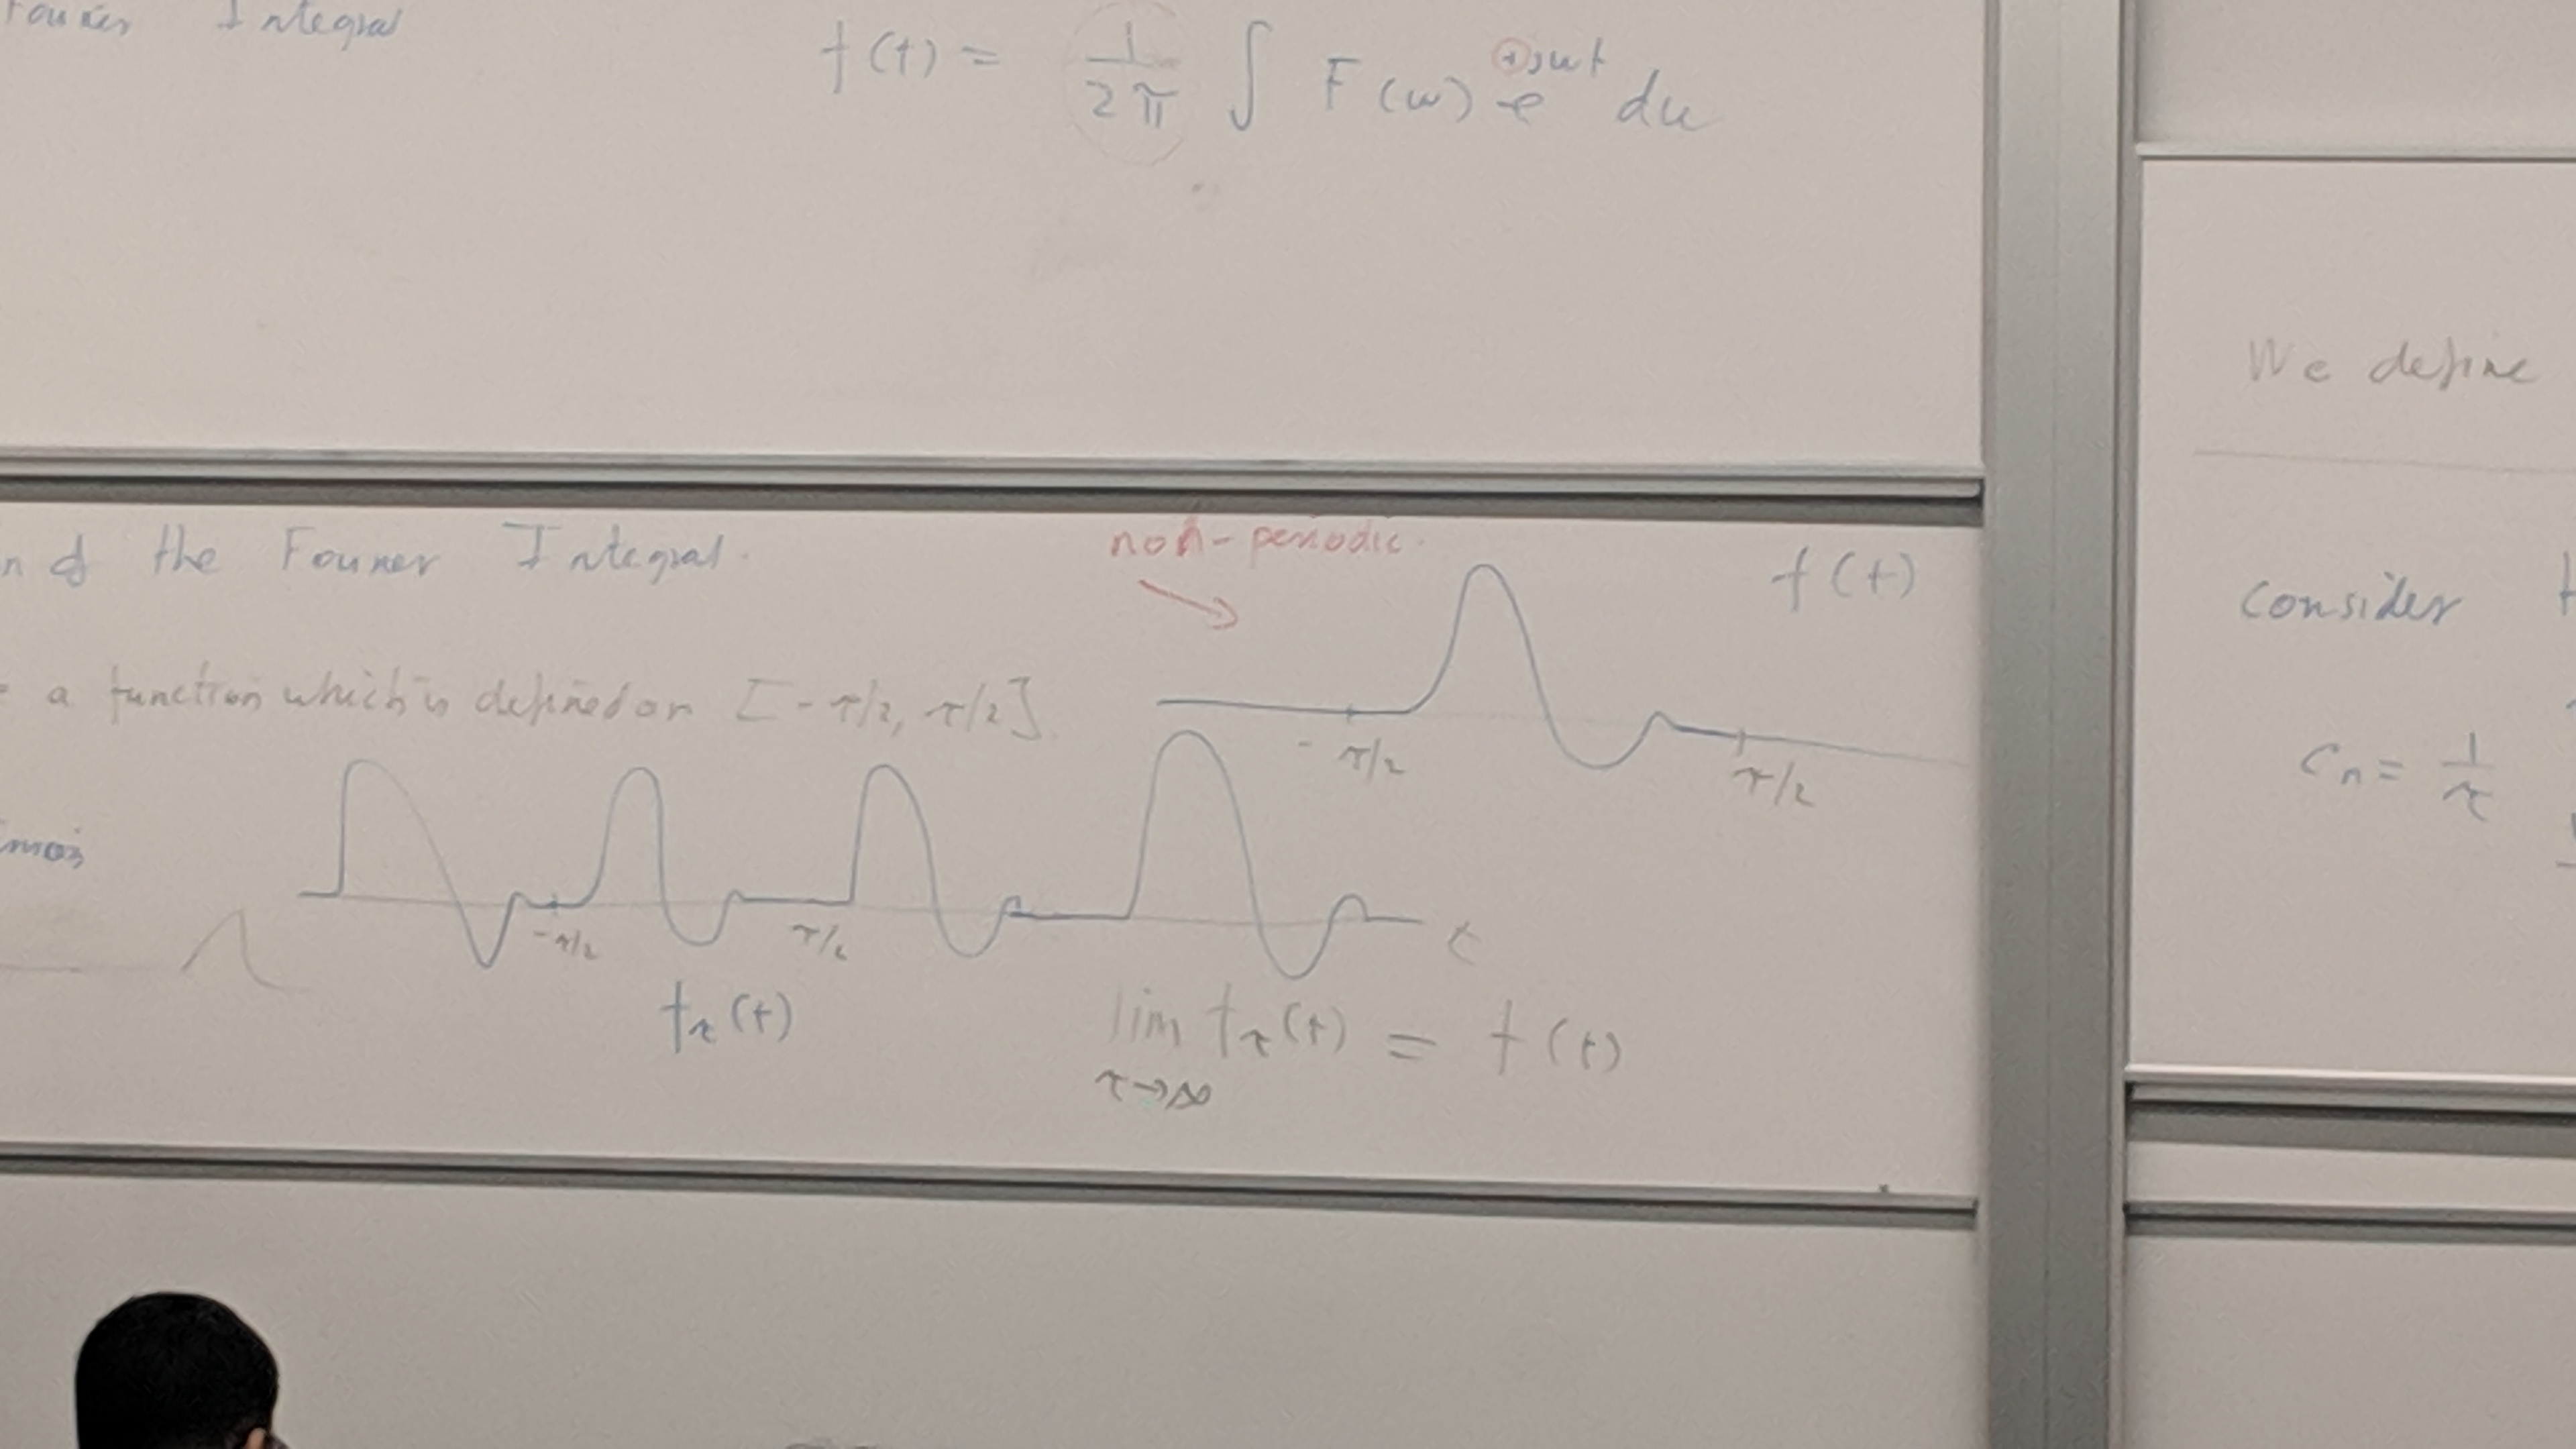
\includegraphics[width=0.8\textwidth]{non-periodic.jpeg}\\

We define
$$F(\omega) =  \int^{\infty}_{-\infty} f(t) e^{-j\omega t}dt $$
Consider the complex Fourier series $f_\tau (t)$
$$\lim_{\tau\to\infty} f_\tau(t) = f(t)$$\\
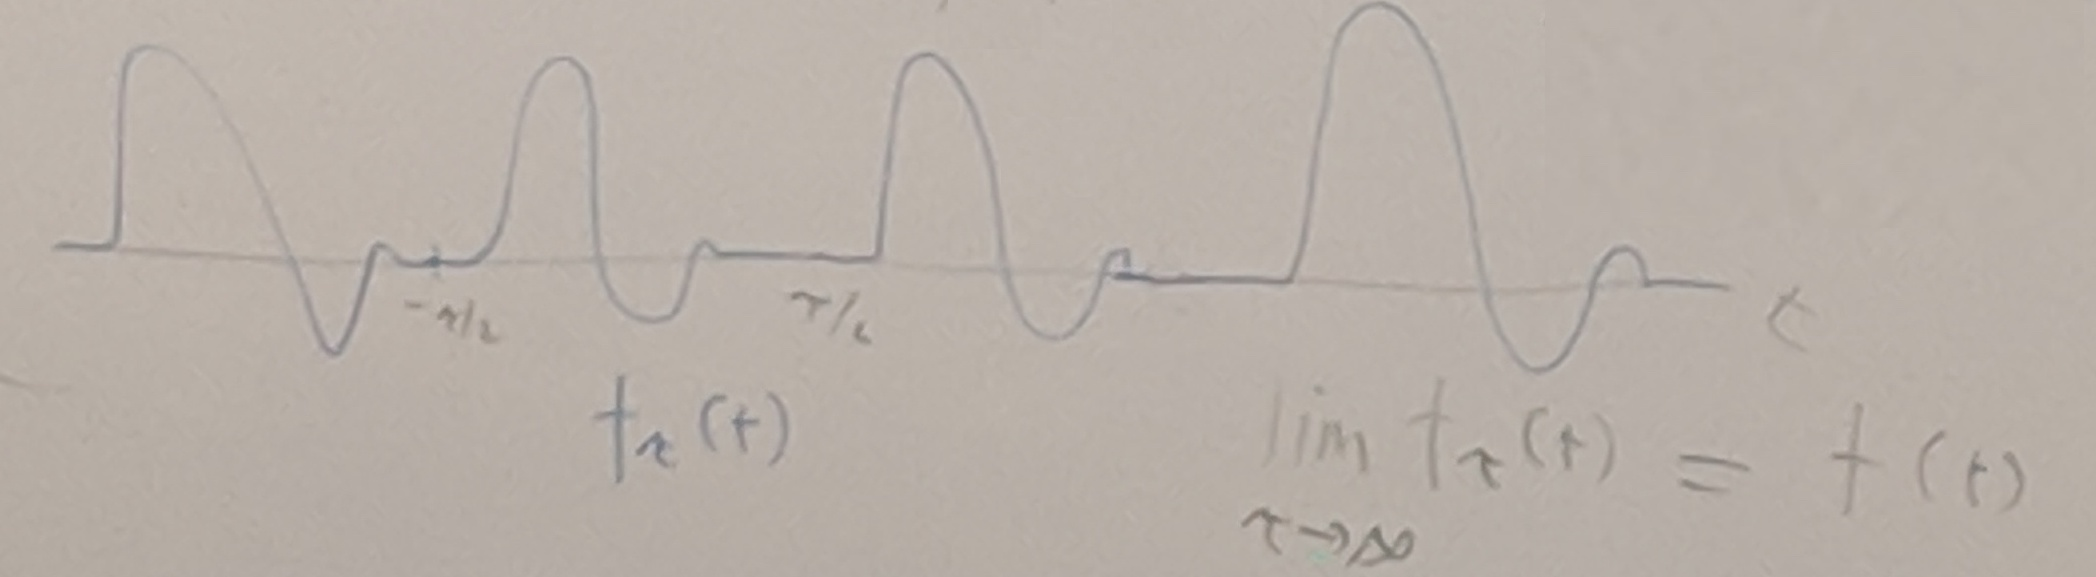
\includegraphics[width=0.8\textwidth]{periodic.jpg}\\

We let $\tau$ to tend to $\infty$ because of that $\omega = \frac{2\pi}{\tau} = \Delta \omega$
$$C_n = \frac{1}{\tau} \int^{\frac{\tau}{2}}_{\frac{-\tau}{2}}f_\tau (t) e^{-jn\omega_0 t}dt$$
$$f_\tau(t) = \sum_{n = -\infty}^\infty C_ne^{jn\omega_0t}$$
$$C_n = \frac{1}{\tau}f_{\tau}f(t)e^{-jn\omega_0 t}dr = \frac{1}{\tau}F(n\omega_0) = \frac{1}{\tau}n\Delta\omega$$
$$f_\tau(t) = \sum_{n = -\infty}^\infty \frac{1}{\tau}F(n\Delta\omega)e^{jn\omega_0t} = \frac{1}{2\pi}\sum_{n = -\infty}^\infty F(n\Delta\omega)e^{jn\omega_0t}\Delta\omega $$
$$[\text{Riemann Sum: }\lim_{N\to\infty, \Delta t \to 0} \sum_{n = 1}^N g(a+n\Delta t) \Delta t = \int_a^b g(t)dt \text{ where } b = a + n\Delta t]$$
$$\lim_{\tau \to \infty} f_\tau (t) = \frac{1}{2\pi}\lim_{\tau \to \infty, \Delta\omega \to 0}\sum_{n=-\infty}^\infty F(n\Delta\omega)e^{jtn\Delta \omega}\Delta \omega = \frac{1}{2\pi}\int^\infty_{-\infty}F(\omega)  e^{jt\omega}d\omega$$
$$ = \int_{-\infty}^{\infty}F(\omega)e^{jt\omega}\;\; \text{ which is known as the Fourier Integral}$$


\end{document}
